% main.tex: write-up of the ECN 593 applied project.
% This folder is a self-contained Overleaf project (compiler: XeLaTeX; set by
% latexmkrc). Locally, compile from writeup/: latexmk main.tex
% Figures in figures/ are byte copies of the code's figures
% (scripts/sync_writeup_figures.py; checked by tests/test_writeup_figures.py).
% This text describes the code on branch main and the committed results.
% If the text and the code disagree, the code is what ran.
% Draft, October 2026.
\documentclass[11pt]{article}

\usepackage[letterpaper,margin=22mm]{geometry}
\usepackage{fontspec}
% DejaVu Sans Mono ships with TeX Live (and Overleaf). Menlo derives from it.
\setmainfont{DejaVuSansMono}[
  Extension=.ttf,
  UprightFont=*,
  BoldFont=*-Bold,
  ItalicFont=*-Oblique,
  BoldItalicFont=*-BoldOblique,
  Scale=0.86,
  Ligatures=TeX,
]
\usepackage{amsmath,amssymb,amsthm}
\usepackage{booktabs}
\usepackage{array}
\usepackage{tabularx}
\usepackage{enumitem}
\usepackage{graphicx}
\usepackage{microtype}
\usepackage{setspace}
\usepackage{titlesec}
\usepackage{needspace}
\usepackage{tikz}
\usetikzlibrary{arrows.meta,positioning,fit,calc,chains}
\usepackage{capt-of}
\usepackage{xcolor}
\usepackage[hidelinks]{hyperref}

\graphicspath{{figures/}}
% Every result number is a macro from numbers.tex (scripts/write_numbers.py).
% numbers.tex: GENERATED by scripts/write_numbers.py from config/ and results/.
% Do not edit by hand. Rerun the script after any run.

\newcommand{\NAgents}{800}
\newcommand{\KSeeded}{80}
\newcommand{\SeedShare}{0.1}
\newcommand{\SeedSharePct}{10}
\newcommand{\Horizon}{20}
\newcommand{\EdgeRate}{4}
\newcommand{\BoxAlphaLo}{-2.5}
\newcommand{\BoxAlphaHi}{-0.5}
\newcommand{\BoxBetaLo}{0.05}
\newcommand{\BoxBetaHi}{0.60}
\newcommand{\BoxGammaLo}{0.05}
\newcommand{\BoxGammaHi}{0.80}
\newcommand{\BoxKappaLo}{0.25}
\newcommand{\BoxKappaHi}{2.50}
\newcommand{\BoxSigmaLo}{0.01}
\newcommand{\BoxSigmaHi}{0.40}
\newcommand{\EtaOne}{0.05}
\newcommand{\EtaTwo}{0.10}
\newcommand{\EtaThree}{0.02}
\newcommand{\CStarAlpha}{-1.5}
\newcommand{\CStarBeta}{0.325}
\newcommand{\CStarGamma}{0.425}
\newcommand{\CStarKappa}{1.375}
\newcommand{\CStarSigma}{0.205}
\newcommand{\RepsEstimand}{200}
\newcommand{\RepsMoment}{30}
\newcommand{\RepsZ}{200}
\newcommand{\ThetaSample}{400}
\newcommand{\WavePoints}{1000}
\newcommand{\WavePointsComma}{1,000}
\newcommand{\PointsEvaluated}{3,000}
\newcommand{\BoxInflationPct}{20}
\newcommand{\Confidence}{0.95}
\newcommand{\ConfidencePct}{95}
\newcommand{\DeltaOne}{0.02}
\newcommand{\DeltaTwo}{0.05}
\newcommand{\DeltaThree}{0.02}
\newcommand{\ShareCut}{0.25}
\newcommand{\StratumMinN}{20}
\newcommand{\ExposureDraws}{10,000}
\newcommand{\CheckPanels}{200}
\newcommand{\GateTruth}{0.03}
\newcommand{\MeanDegree}{8.085}
\newcommand{\MeanDegreeTheory}{7.97}
\newcommand{\DegreeCut}{12}
\newcommand{\DegreeCutTotal}{36}
\newcommand{\DegreeCutSeeded}{35}
\newcommand{\Tau}{7.8147}
\newcommand{\ZOne}{0.2638}
\newcommand{\ZTwo}{0.05}
\newcommand{\ZThree}{0.2618}
\newcommand{\WaveKeptOne}{202}
\newcommand{\WaveKeptTwo}{416}
\newcommand{\WaveKeptThree}{373}
\newcommand{\NNroy}{991}
\newcommand{\WaveMinIOne}{0.0017}
\newcommand{\WaveMinITwo}{0.0050}
\newcommand{\WaveMinIThree}{0.0071}
\newcommand{\WaveMedIOne}{50.37}
\newcommand{\WaveMedITwo}{11.89}
\newcommand{\WaveMedIThree}{13.59}
\newcommand{\MinI}{0.0017}
\newcommand{\MedI}{2.0208}
\newcommand{\MinIAlpha}{-1.4871}
\newcommand{\MinIBeta}{0.399}
\newcommand{\MinIGamma}{0.3301}
\newcommand{\MinIKappa}{1.3446}
\newcommand{\MinISigma}{0.1984}
\newcommand{\MedIKappa}{2.4654}
\newcommand{\ThetaOneStar}{0.03631}
\newcommand{\ThetaTwoStar}{0.03826}
\newcommand{\ThetaTwoStarShort}{0.0383}
\newcommand{\PremiumStar}{0.00195}
\newcommand{\SpillStar}{0.00792}
\newcommand{\ThetaHmLo}{0.00587}
\newcommand{\ThetaHmHi}{0.07325}
\newcommand{\ThetaHmLoShort}{0.0059}
\newcommand{\ThetaHmHiShort}{0.0732}
\newcommand{\ThetaExpLo}{-0.000571}
\newcommand{\ThetaExpHi}{0.026893}
\newcommand{\RecheckHmLoIndex}{877}
\newcommand{\RecheckHmLoPilot}{+0.005870}
\newcommand{\RecheckHmLoPilotSE}{0.000004}
\newcommand{\RecheckHmLoFresh}{+0.005871}
\newcommand{\RecheckHmLoFreshSE}{0.000003}
\newcommand{\RecheckHmHiIndex}{802}
\newcommand{\RecheckHmHiPilot}{+0.073250}
\newcommand{\RecheckHmHiPilotSE}{0.000006}
\newcommand{\RecheckHmHiFresh}{+0.073255}
\newcommand{\RecheckHmHiFreshSE}{0.000006}
\newcommand{\RecheckExpLoIndex}{944}
\newcommand{\RecheckExpLoPilot}{-0.000571}
\newcommand{\RecheckExpLoPilotSE}{0.000502}
\newcommand{\RecheckExpLoFresh}{+0.000201}
\newcommand{\RecheckExpLoFreshSE}{0.000491}
\newcommand{\RecheckExpHiIndex}{904}
\newcommand{\RecheckExpHiPilot}{+0.026893}
\newcommand{\RecheckExpHiPilotSE}{0.000259}
\newcommand{\RecheckExpHiFresh}{+0.027274}
\newcommand{\RecheckExpHiFreshSE}{0.000263}
\newcommand{\RecheckExpLoFreshAbs}{0.000201}
\newcommand{\MinIThetaTwo}{0.03708}
\newcommand{\MedIThetaTwo}{0.06346}
\newcommand{\MinIThetaTwoShort}{0.0371}
\newcommand{\MinIFoilOneLo}{0.03259}
\newcommand{\MinIFoilOneHi}{0.03465}
\newcommand{\MedIFoilOneLo}{0.05832}
\newcommand{\MedIFoilOneHi}{0.05949}
\newcommand{\MinIBetaHat}{0.3362}
\newcommand{\MedIBetaHat}{0.5890}
\newcommand{\MinIBetaLo}{0.3259}
\newcommand{\MinIBetaHi}{0.3465}
\newcommand{\MedIBetaLo}{0.5832}
\newcommand{\MedIBetaHi}{0.5949}
\newcommand{\MinIFoilOneBelowPct}{9.3}
\newcommand{\MedIFoilOneBelowPct}{7.2}
\newcommand{\MinISpill}{0.00613}
\newcommand{\MedISpill}{0.00809}
\newcommand{\MinISpillShort}{0.0061}
\newcommand{\MinIFoilTwoEst}{0.00619}
\newcommand{\MinIFoilTwoSE}{0.00470}
\newcommand{\MedIFoilTwoEst}{0.00826}
\newcommand{\MedIFoilTwoSE}{0.00416}
\newcommand{\MinIFoilTwoLo}{-0.003022}
\newcommand{\MinIFoilTwoHi}{0.015410}
\newcommand{\MedIFoilTwoLo}{0.000112}
\newcommand{\MedIFoilTwoHi}{0.016406}
\newcommand{\MinISeededPart}{0.03374}
\newcommand{\MinIUnseededPart}{0.00333}
\newcommand{\MinISeededContrast}{0.3374}
\newcommand{\MinIMeanBeta}{0.3339}
\newcommand{\MinIGapMeanBeta}{0.00369}
\newcommand{\MinIUnseededShareMeanBeta}{0.9034}
\newcommand{\MinIOlsErrorPart}{0.00036}
\newcommand{\MinIGapDisplayed}{0.00346}
\newcommand{\MinIUnseededShareDisplayed}{0.9642}
\newcommand{\MinIBaselineGap}{0.0007}
\newcommand{\MinIUnseededShareDisplayedPct}{96}
\newcommand{\MedISeededPart}{0.05925}
\newcommand{\MedIUnseededPart}{0.00421}
\newcommand{\MedISeededContrast}{0.5925}
\newcommand{\MedIMeanBeta}{0.5880}
\newcommand{\MedIGapMeanBeta}{0.00466}
\newcommand{\MedIUnseededShareMeanBeta}{0.9027}
\newcommand{\MedIOlsErrorPart}{0.00045}
\newcommand{\MedIGapDisplayed}{0.00456}
\newcommand{\MedIUnseededShareDisplayed}{0.9236}
\newcommand{\MedIBaselineGap}{0.0007}
\newcommand{\MedIUnseededShareDisplayedPct}{92}
\newcommand{\UnseededShareMeanBetaPct}{90}
\newcommand{\GateAssignments}{10,000}
\newcommand{\GateMeanEstimate}{0.03006}
\newcommand{\GateRatio}{1.034}
\newcommand{\GateRatioBootSE}{0.0154}
\newcommand{\GateCoveragePct}{93.4}
\newcommand{\GateCoverageLoPct}{92.9}
\newcommand{\GateCoverageHiPct}{93.9}
\newcommand{\KernelCovStar}{0.920}
\newcommand{\KernelCovMinI}{0.930}
\newcommand{\KernelCovMedI}{0.925}
\newcommand{\DesignCovStar}{0.930}
\newcommand{\DesignCovMinI}{0.930}
\newcommand{\DesignCovMedI}{0.9267}
\newcommand{\WbZOne}{0.8621}
\newcommand{\WbZTwo}{0.6054}
\newcommand{\WbZThree}{0.6864}
\newcommand{\WbZTwoShort}{0.61}
\newcommand{\WbBestI}{204.35}
\newcommand{\WbMedianI}{1093.22}
\newcommand{\WbMaxI}{1818.34}
\newcommand{\WbClosestMOne}{0.6188}
\newcommand{\WbClosestMTwo}{0.0545}
\newcommand{\WbClosestMThree}{0.6133}
\newcommand{\WbClosestMTwoShort}{0.05}


\definecolor{ink}{HTML}{111111}
\definecolor{rule}{HTML}{222222}
\definecolor{wash}{HTML}{F4F4F4}
\definecolor{line}{HTML}{555555}

\setstretch{1.12}
\pagestyle{plain}
\setlength{\parindent}{0pt}
\setlength{\parskip}{0.55em}
\setlist[itemize]{leftmargin=1.4em,itemsep=0.15em,topsep=0.25em}
\setlist[enumerate]{leftmargin=1.6em,itemsep=0.15em,topsep=0.25em}

\titleformat{\section}[block]
  {\needspace{8\baselineskip}\normalsize\bfseries\color{ink}}
  {\thesection}{0.7em}{}
  [\vspace{-0.4em}{\color{rule}\titlerule[0.4pt]}]
\titleformat{\subsection}[runin]
  {\normalsize\bfseries\color{ink}}
  {\thesubsection}{0.6em}{}[.~]
\titlespacing*{\section}{0pt}{1.4em}{0.7em}
\titlespacing*{\subsection}{0pt}{0.9em}{0.4em}

\newcommand{\NROY}{\mathrm{NROY}}
\newcommand{\hm}{\mathrm{hm}}
\newcommand{\expset}{\mathrm{exp}}
\newcommand{\prem}{\psi}
\newcommand{\interior}{\operatorname{int}}
\newcommand{\Jone}{J_1}
\newcommand{\Jtwo}{J_2}
\newcommand{\dspill}{\delta_{\mathrm{spill}}}
\newcommand{\ddir}{\delta_{\mathrm{dir}}}

\begin{document}

\hypersetup{pageanchor=false}
% cover.tex: the cover page of the ECN 593 final report.
% Every result number is a macro from numbers.tex (scripts/write_numbers.py).
% The diagram uses data coordinates. The axis ranges and label offsets are
% layout: check the cover by eye after a rerun that moves a value.
\begin{titlepage}
\thispagestyle{empty}
\setlength{\parskip}{0pt}
\raggedright

{\footnotesize\color{line}%
ECN 593 \textperiodcentered\ APPLIED PROJECT \textperiodcentered\ FINAL REPORT\hfill ARIZONA STATE UNIVERSITY\par}
\vspace{0.5em}
{\color{rule}\rule{\linewidth}{1.2pt}}
\vspace{1.2em}

{\fontsize{24}{29}\selectfont\bfseries\color{ink}%
Not-ruled-out images\\[0.15em]of policy contrasts\par}
\vspace{0.9em}
{\normalsize\color{line}%
A village agent-based model, calibrated by history matching,\\
and two analysts (a field experimenter and a calibrator)\\
graded against what the targets cannot rule out\par}

\vspace{1.2em}

% ---- the paper in one picture: the min-I point (the best-fitting NROY point)
{\normalsize\bfseries\color{ink} The paper in one picture\par}
\vspace{0.7em}
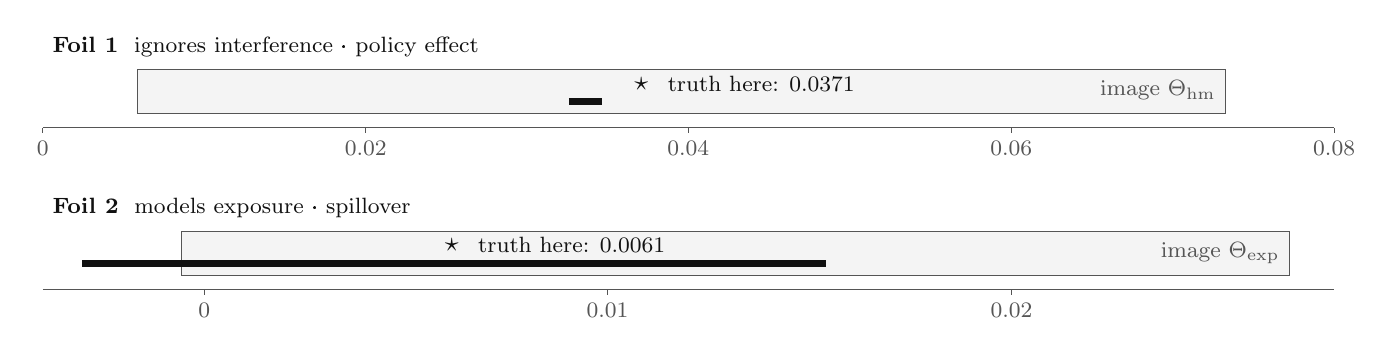
\begin{tikzpicture}[
    every node/.style={font=\footnotesize, text=ink},
    band/.style={fill=wash, draw=line, line width=0.3pt},
    foil/.style={line width=2.4pt, draw=ink},
    truth/.style={font=\normalsize},
    tick/.style={line width=0.4pt, draw=line}]
  % Row 1: theta_2 on [0, 0.08] mapped to 16.4 cm (x = 205 cm per unit)
  \begin{scope}[x=205cm, y=1cm]
    \node[anchor=south west] at (0, 0.78) {\bfseries Foil 1\normalfont\ \ ignores interference \textperiodcentered\ policy effect};
    \fill[band] (\ThetaHmLo, 0.18) rectangle (\ThetaHmHi, 0.74);
    \node[anchor=north east, text=line] at (\ThetaHmHi, 0.72) {image $\Theta_{\mathrm{hm}}$};
    \draw[foil] (\MinIFoilOneLo, 0.33) -- (\MinIFoilOneHi, 0.33);
    \node[truth] (star1) at (\MinIThetaTwo, 0.56) {$\star$};
    \node[anchor=west] at (star1.east) {truth here: \MinIThetaTwoShort};
    \draw[tick] (0, 0) -- (0.08, 0);
    \foreach \v in {0, 0.02, 0.04, 0.06, 0.08} {
      \draw[tick] (\v, 0) -- (\v, -0.07);
      \node[below, text=line] at (\v, -0.05) {\v};}
  \end{scope}
  % Row 2: delta_spill on [-0.004, 0.028] mapped to 16.4 cm (x = 512.5 cm per unit)
  \begin{scope}[x=512.5cm, y=1cm, xshift=2.05cm, yshift=-2.05cm]
    \node[anchor=south west] at (-0.004, 0.78) {\bfseries Foil 2\normalfont\ \ models exposure \textperiodcentered\ spillover};
    \fill[band] (\ThetaExpLo, 0.18) rectangle (\ThetaExpHi, 0.74);
    \node[anchor=north east, text=line] at (\ThetaExpHi, 0.72) {image $\Theta_{\mathrm{exp}}$};
    \draw[foil] (\MinIFoilTwoLo, 0.33) -- (\MinIFoilTwoHi, 0.33);
    \node[truth] (star2) at (\MinISpill, 0.56) {$\star$};
    \node[anchor=west] at (star2.east) {truth here: \MinISpillShort};
    \draw[tick] (-0.004, 0) -- (0.028, 0);
    \foreach \v in {0, 0.01, 0.02} {
      \draw[tick] (\v, 0) -- (\v, -0.07);
      \node[below, text=line] at (\v, -0.05) {\v};}
  \end{scope}
\end{tikzpicture}

\vspace{0.4em}
{\footnotesize\color{line}%
The diagram shows the min-I point, the calibrator's best-fitting NROY point. The two
rows use different scales. Bands: the image of the effect over \ThetaSample{} sampled NROY points. Black
lines: the analyst's nominal \ConfidencePct\% interval from one panel. Stars: the
simulator's true value at this point. Foil~1 is tight, sits inside the band,
and misses the truth. Foil~2 contains the truth, yet it also sits inside its
band: narrower than what the targets leave open.\par}

\vspace{0.9em}

% ---- question and answer
\noindent
\begin{minipage}[t]{0.47\linewidth}\raggedright
{\normalsize\bfseries\color{ink} The question}\par\vspace{0.4em}
{\small Many parameter points fit the same \NMoments{} targets (the status quo plus
one randomized pilot), and they imply different effects of seeding the
hubs. What must a calibrated simulator report? How far can an interval
computed at one point be trusted?\par}
\end{minipage}\hfill
\begin{minipage}[t]{0.47\linewidth}\raggedright
{\normalsize\bfseries\color{ink} The answer}\par\vspace{0.4em}
{\small In the one panel at each point, Foil~1 misses the truth at all
three points, the real village included, and is F-OVERCONF at all three.
Foil~2 contains the truth at all three, and is F-OVERCONF at both
calibrated points; at the real village it has no verdict. Report the image,
not one point.\par}
\end{minipage}

\vspace{0.9em}

% ---- in numbers
{\normalsize\bfseries\color{ink} In numbers\par}
\vspace{0.4em}
{\footnotesize
\begin{tabularx}{\linewidth}{@{}X r@{}}
\toprule
\textcolor{line}{Points evaluated in three history-matching waves / points kept (NROY)} & \PointsEvaluated{} / \NNroy{} \\
\textcolor{line}{Image of the policy effect over the sampled NROY points} & [\ThetaHmLoShort, \ThetaHmHiShort] \\
\textcolor{line}{Policy effect at the planted point c*} & \ThetaTwoStarShort{} \\
\textcolor{line}{Foil 1 estimate below the truth, at $c^\star$ / min-I / median-I} & \StarPtFoilOneBelowPct\% / \MinIFoilOneBelowPct\% / \MedIFoilOneBelowPct\% \\
\textcolor{line}{Foil 2 interval coverage when the exposure map holds exactly} & \GateCoveragePct\% \\
\bottomrule
\end{tabularx}\par}

\vfill

{\color{rule}\rule{\linewidth}{0.4pt}}\par\vspace{0.6em}
\noindent
\begin{minipage}[t]{0.44\linewidth}\raggedright
{\small\bfseries\color{ink} Augusto Gonz\'alez-Bonorino}\par\vspace{0.15em}
{\footnotesize\color{line} Arizona State University\\
Applied project for ECN 593\par}
\end{minipage}\hfill
\begin{minipage}[t]{0.54\linewidth}\raggedleft
{\footnotesize\color{line} Draft for review, October 2026\\
\texttt{github.com/Bonorinoa/ecn593-applied-project}\\
Deterministic \textperiodcentered\ 55 tests \textperiodcentered\ one command replicates it\par}
\end{minipage}
\end{titlepage}

\hypersetup{pageanchor=true}

\noindent
A calibrated simulator gives a policy effect for each parameter point
that fits the targets. Many points fit the targets equally well, yet
they imply different effects. This note therefore reports the
\emph{image} of the policy effect over the sampled NROY points, not one
number. The image follows the \emph{reporting logic} of a partially
identified set (Manski 2003, Tamer 2010), though it is not an identified set in their
sense (Sections~\ref{sec:pi} and~\ref{sec:not}).

The targets are what a researcher could observe: the village in the
status quo, plus one randomized pilot. The policy we want to predict,
seeding the highest-degree people, is never a target. We then ask two
analysts for an interval. The \emph{field experimenter} has one panel
from the real village, and her test is whether her interval is right
about her own world. The \emph{calibrator} fits the model and works at
one best-fitting point, and her tests are whether her interval is right
about the real village and how it sits against the image. Because the
targets are planted, the true effect is known, and the test can grade
both analysts.

% HEADLINE CANDIDATE (v2), written from the results by the writer card W1
% and revised by W2 for G1 FIX-5a (one panel). It is NOT yet adopted:
% Augusto decides (see the W2 handoff).
\medskip
\noindent\textbf{Headline.}
\begin{quote}
In the one panel at each point, Foil 1 misses the truth at all three
points, the real village included, and is F-OVERCONF at all three. Foil 2
contains the truth at all three points, and is F-OVERCONF at both
calibrated points; at the real village it has no verdict. Report the
image, not one point.
\end{quote}
The analyst who ignores interference reports a tight interval that sits
inside the image and misses the truth, even before any calibration. The
analyst who models exposure contains the truth at all three points, in that one panel, yet at both
calibrated points her interval is strictly narrower than the set of
spillovers that the targets leave open.

The model is a village of \NAgents{} people on a fixed random graph, and
each person has a preventive-behavior level in $(0,1)$. A campaign seeds
\SeedSharePct\% of the people. Section~\ref{sec:results} gives the
numbers.

%----------------------------------------------------------------
\section{The planner's problem}

A planner compares assignment rules (policies) that act on people who
influence each other. Under interference, the outcome of person $i$
depends on the whole assignment vector, so the effect of treating person
$i$ alone is not defined. The natural estimand is a contrast of rules,
\begin{equation}
  \theta(\pi,\pi';c)
  \;=\;
  \mathbb{E}_c\!\left[\bar Y_T(\pi)\right]
  \;-\;
  \mathbb{E}_c\!\left[\bar Y_T(\pi')\right].
\end{equation}
Here $c$ indexes a complete data-generating process (a kernel), and the
expectation is over the simulation noise that remains once $c$ is fixed.

The planner does not know $c$. She has a class of kernels $\{f(\,\cdot\,;c):c\in C\}$ and a
short vector of moments $z$ that she wants to match. History matching
then \emph{rules out} parameter points; it does not give a posterior
over $c$. The decision-relevant object is not the kept set in parameter
space but the image of $\theta$ over that set.

Two sources of doubt sit side by side, and we keep them apart. The first
is calibration: which parameter points remain. The second is the
analyst: a default estimator fits one panel at one parameter point. For
each analyst we report an interval and compare it with the truth and
with its own image.

%----------------------------------------------------------------
\section{Objects}

\paragraph{World, kernel and panel.}
The world is the graph $A$ plus the covariates $X$. It is drawn once,
and every simulation shares it. The kernel $f$ maps a parameter point
$c$, simulation noise $\omega$ and an assignment rule $\pi$ to a panel $(Y_T,D)$. The
kernel is complete, in that it can run every arm on the same noise, and
the incompleteness lives in $c$, not in unobserved counterfactuals
inside $f$ (Section~\ref{sec:po}). The code implements the kernel as
vectorized algebra (\texttt{simulate\_panel} in \texttt{kernel.py}).

One run of the kernel gives one panel,
\begin{equation}
  \mathcal{D}(c,\omega,\pi)
  \;=\;
  \bigl\{(Y_{iT},\,D_i,\,X_i,\,A_{i\cdot})\bigr\}_{i=1}^{N}.
\end{equation}
A parameter point is not a panel: one panel is one draw of $\omega$. The
kernel truth $\theta(c)$ uses $R=\RepsEstimand$ paired reps, whereas an analyst sees
one panel.

\paragraph{Box.}
$C\subset\mathbb{R}^5$ is the a priori range of the free parameters $c=(\alpha,\beta,\gamma,\kappa,\sigma_\varepsilon)$. The vector $\eta$ is
fixed inside the kernel and is not in $C$.

\paragraph{Estimands.}
Let $\bar Y_T$ be the mean of $Y_T$ over people. The code defines three
estimands:
\begin{align}
  \theta_1(c)
  &= \mathbb{E}_c[\bar Y_T\mid\pi_1]-\mathbb{E}_c[\bar Y_T\mid\pi_0],
  \\
  \theta_2(c)
  &= \mathbb{E}_c[\bar Y_T\mid\pi_2]-\mathbb{E}_c[\bar Y_T\mid\pi_0]
  \quad\text{(headline)},
  \\
  \prem(c)
  &= \theta_2(c)-\theta_1(c)
  \quad\text{(the premium)}.
\end{align}
The arm $\pi_0$ seeds no one (control, the status quo), the arm $\pi_1$ seeds \KSeeded{} people
at random (random arm, the pilot), and the arm $\pi_2$ seeds the \KSeeded{} people with
the highest degree (degree arm, the policy to predict). The expectation is over simulation
noise and over the random assignment in $\pi_1$. The code replaces each
expectation with a mean over \RepsEstimand{} paired reps, and we define
$\theta$ on the terminal mean $\bar Y_T$, not on the path.

Two exposure contrasts, $\dspill(c)$ and $\ddir(c)$, are defined with the foils
(Section~\ref{sec:design}). The letter $\tau$ is only the threshold, and
the premium is $\prem$.

\paragraph{Moments and targets.}
$M:C\to\mathbb{R}^{\NMoments}$ is the map from a parameter point to \NMoments{} simulated summaries
(Section~\ref{sec:targets}). The
targets $z\in\mathbb{R}^{\NMoments}$ are the values that $M(c)$ must match. With five free
parameters and \NMoments{} moments, the model is underidentified on purpose:
the question is which policy effects remain possible, not which $c$ is
true.

\paragraph{Implausibility.}
\begin{equation}
  I(c)
  \;=\;
  \bigl(z-\widehat M(c)\bigr)^{\!\top}
  V(c)^{-1}
  \bigl(z-\widehat M(c)\bigr),
  \qquad
  V(c)=\mathrm{diag}\bigl(\sigma^2_z+\sigma^2_{\mathrm{MC}}(c)+\delta^{\circ 2}\bigr).
\end{equation}
$I(c)$ is a variance-weighted sum of squared gaps, not a distance. The
three terms in $V$ are the Monte Carlo variance of the targets, the
Monte Carlo variance of the candidate moment, and a model-error
allowance, which we call the discrepancy $\delta$.

\paragraph{NROY.}
In the code, NROY is a finite set: the union, over three Latin-hypercube
waves, of the sampled points $c$ with $I(c)\le\tau$. It approximates
the level set $\{c\in C:I(c)\le\tau\}$ but does not enumerate it.
Membership means we cannot rule out $c$. It does not mean that $c$ equals the truth. NROY is not a
posterior.

\paragraph{Images.}
\begin{align}
  \Theta_{\hm}
  &= \{\theta_2(c):c\in\mathcal S\},
  &
  \Theta_{\expset}
  &= \{\dspill(c):c\in\mathcal S\},
\end{align}
where $\mathcal S$ is a declared uniform sample of \ThetaSample{} NROY points. The
code reports each image as the range $[L,U]$ over $\mathcal S$: the
declared empirical image. The range is not a distribution. Different NROY
points can give different values of $\theta_2$, but they need not.

\paragraph{Diagnostic points.}
There are three diagnostic points, and we write $c_0$ for any of them.
The min-I point and the median-I point of NROY belong to the calibrator.
Both depend on $I$ only, never on $\theta$. The third point is
$c^\star$, the real village, and it belongs to the field experimenter
(Section~\ref{sec:twoanalysts}).

\paragraph{Foils.}
A foil is an estimator that an analyst fits on one panel at a diagnostic point
$c_0$. Each foil is judged against the truth at $c_0$, against the truth at $c^\star$,
and against its own image (Sections~\ref{sec:geometry} and~\ref{sec:twoanalysts}). A foil never sees NROY, so it is not a
candidate for $\Theta_{\hm}$.

%----------------------------------------------------------------
\section{Potential outcomes, and what counts as data}
\label{sec:po}

Under SUTVA, $Y_i=Y_i(D_i)$ with $D_i\in\{0,1\}$. One of the two
numbers per person is missing. That missing number is the
incompleteness in the data. A regression with robust standard errors
quantifies within-point uncertainty under the analyst's stated
assumptions. It is a ruler, not a villain.

This project drops SUTVA: peers influence each other through outcomes
($\gamma>0$), so $Y_i=Y_i(\mathbf{d})$ with $\mathbf{d}\in\{0,1\}^N$. The contrast $Y_i(1)-Y_i(0)$ is not defined unless the
assignment of everyone else is named. The well-defined object is an
overall policy contrast in the sense of Hudgens and Halloran (2008), namely $\theta(\pi,\pi';c)$ from Section~1.

In the field, the other values of $\bar Y(\pi)$ are missing because there is one
campaign. In the simulator, $f$ is complete: run both arms on
paired noise and subtract. What remains unknown is which $c\in C$ is right,
so $\Theta_{\hm}$ is a not-ruled-out image. It is not a Manski identified set, and
it is not a set of possible $Y_i(0)$. It shares the \emph{reporting logic}
(do not replace a set by a convenient point) but not the theorem.

\paragraph{Only two objects have empirical analogs.}
\begin{center}
\small
\begin{tabular}{@{}llp{52mm}@{}}
\toprule
empirical analog & simulator object & who uses it \\
\midrule
micro data of one campaign
  & one panel $\mathcal{D}(c,\omega,\pi)$
  & Foil 1, Foil 2 \\
status-quo data and one pilot
  & $z$ with its variances and $\delta$
  & $I(c)$, $\NROY$ \\
\bottomrule
\end{tabular}
\end{center}
The following objects are not data: the Latin-hypercube points, the
Monte Carlo reps, the NROY points, the image sample and $\theta(c)$. They are
probes of $f$, and NROY points are arguments of $\theta(\cdot)$, not extra surveys.

%----------------------------------------------------------------
\section{The targets: the status quo and one randomized pilot}
\label{sec:targets}

The targets are what a researcher could observe. She sees the village as
it is (the status quo, arm $\pi_0$), and she can run one randomized
pilot (the random arm $\pi_1$). She never sees the degree arm $\pi_2$
beside either of them. That arm is the policy she wants to predict, so
it is never a target. If it were, the targets would contain the answer
to the planner's question.\footnote{The earlier design of this project
did exactly that. Its targets used outcomes under both seeding
policies, and their difference was the targeting premium. It is
archived at the git tag \texttt{v1-worldbank-moments} and is not
described further here.}

The code uses four moments, in a fixed order. Each is a mean over
$R_m=\RepsMoment$ paired reps, and rep $r$ of the control arm and of
the random arm share one state stream.
\begin{center}
\small
\begin{tabular}{@{}rllp{58mm}@{}}
\toprule
\# & name & arm & definition \\
\midrule
1 & \texttt{sq\_level} & control & mean over people of $Y_T$ \\
2 & \texttt{sq\_corr\_x1} & control & corr over people of $(Y_T,x_1)$ \\
3 & \texttt{sq\_peer\_corr} & control & corr over people of $\bigl(Y_{T,i},(WY_T)_i\bigr)$, with $W=A/k_i$ \\
4 & \texttt{pilot\_level} & random & mean over people of $Y_T$ \\
\bottomrule
\end{tabular}
\end{center}
Here $x_1$ is the first covariate and $W$ is the kernel's row-normalized
adjacency, the same peer mean that enters the update rule. The Monte
Carlo variance of each moment is the sample variance over the reps
(with one degree of freedom removed) divided by the number of finite
values. The code drops non-finite correlations. If fewer than two
values are finite, the variance is infinite and $I$ rejects the point.

The targets are planted: $z:=\widehat M(c^\star)=(\ZOne,\,\ZTwo,\,\ZThree,\,\ZFour)$, with \RepsZ{}
reps and its Monte Carlo variances. The file \texttt{data/planted.json}
stores them. Planting supplies a known benchmark and makes a match
plausible. It does not guarantee that a finite Latin-hypercube search
keeps a point. It also makes the true effect known, and that is the only
way to check an overlay.

\paragraph{The discrepancy $\delta$ and the threshold $\tau$.}
The discrepancy is $\delta=(\DeltaOne,\,\DeltaTwo,\,\DeltaThree,\,\DeltaFour)$ in the order above: \DeltaOne{} for the
two levels and \DeltaTwo{} for the two correlations.
The threshold is the \Confidence{} quantile of $\chi^2$ with $\NMoments$
degrees of freedom, one per moment, so $\tau=\Tau$.
The discrepancy is a design tolerance, and it is the binding one for
$\kappa$. On a single coordinate the level allowance is the square root of
$\tau$ times $\delta_1^2$ ($\tau=\Tau$, $\delta_1=\DeltaOne$). That allowance
is larger than $\theta_1(c^\star)=\ThetaOneStar$, so a level match cannot
pin a treatment effect of this size. The spread ratio for $\kappa$ is
\SpreadRatioKappa{} (Section~\ref{sec:spread}). The peer-correlation moment
is a separate failure: \SpreadRatioGamma{} is not a restriction, because the
moment hardly moves with $\gamma$ (a check at $c^\star$, not a committed
result; Section~\ref{sec:spread}). Four moments against five parameters is
not why the image is wide.

\paragraph{The paired-rep identity.}
Because the control and random arms share their state streams,
$\texttt{pilot\_level}-\texttt{sq\_level}$ at $c^\star$ is $\theta_1(c^\star)$
(the two printed values are $\PilotMinusSq$ and $\ThetaOneStar$). This is
intended: a randomized pilot identifies $\theta_1$. The question is
whether the model can extrapolate from the pilot to $\theta_2$, the
effect of seeding the hubs.

\paragraph{What the moments cannot do.}
The moments use two arms, not three, and the control arm appears only as
the status quo. So $\theta_2$, a contrast of the degree arm against
control, is not a moment that the code matches. The code uses fewer
reps for the moments than for the estimands because the search must be
cheap, and the estimands are computed only for kept points. The targets
and the estimands each use \RepsEstimand{} reps. Equal replication
counts do not imply equal Monte Carlo precision across these different
statistics.

%----------------------------------------------------------------
\section{Order of operations}

The order matters: if $\theta$ decides which $c$ to keep, the image is a fit,
not a report. For that reason the code fixes every exogenous parameter
in \texttt{config/} before any wave runs.

\begin{enumerate}
  \item Fix the kernel $f$, the box $C$, the targets $z$, the
        discrepancy $\delta$, the threshold $\tau$, the estimands and
        the rule for the diagnostic points.
  \item Draw the world $(A,X)$ once.
  \item History matching. Evaluate $I(c)$ on a space-filling design and
        keep the points with $I\le\tau$. Later waves search the box of the kept
        points; NROY is the union of the kept points. An empty NROY
        is a finding: the pair $(f,z)$ is rejected. Never move $\tau$ or $\delta$.
  \item Leg~A. Sample \ThetaSample{} NROY points, compute $\theta_2(c)$ and $\dspill(c)$ at
        each, and report $\Theta_{\hm}$ and $\Theta_{\expset}$ as ranges. Then evaluate the
        endpoint candidates again with fresh reps.
  \item Leg~B. At each of the three diagnostic points, fit the two foils on one panel
        and compare each interval with the truth at that point, with the truth at
        $c^\star$, and with its own image.
\end{enumerate}

\vspace{0.6em}
\begin{center}
\begin{minipage}{\linewidth}
\centering
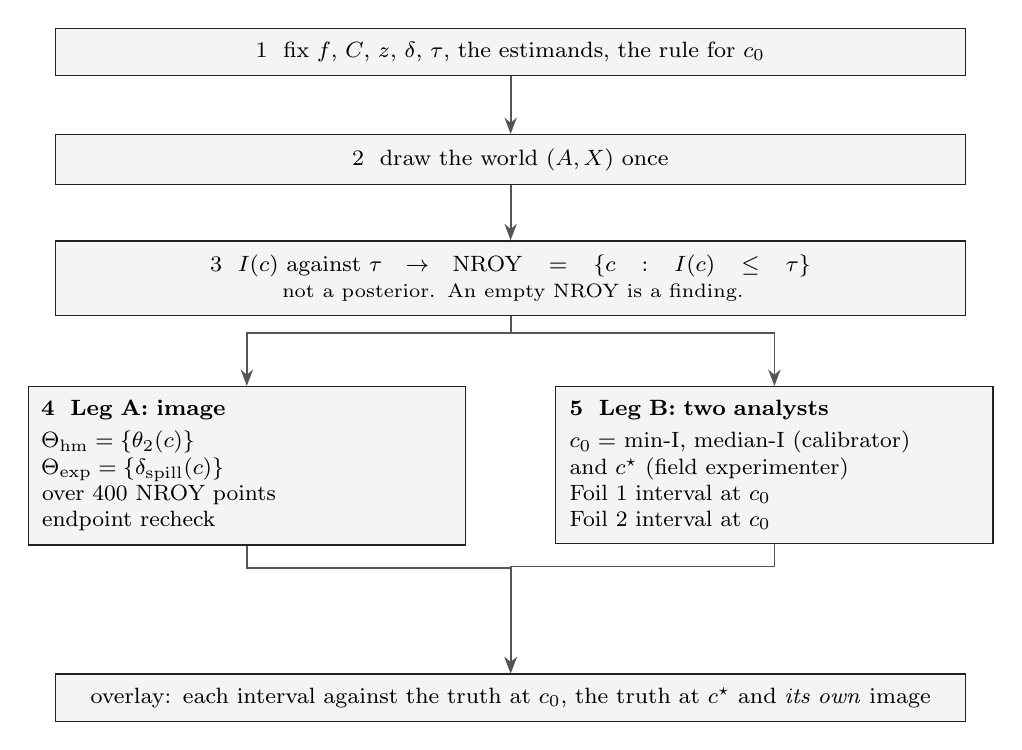
\begin{tikzpicture}[
  font=\footnotesize,
  >=Stealth,
  box/.style={
    draw=rule, line width=0.45pt, fill=wash,
    inner sep=5pt, align=left, anchor=north,
  },
  wide/.style={box, text width=112mm, align=center},
  col/.style={box, text width=52mm},
  arr/.style={->, line width=0.65pt, color=line},
]
  \node[wide] (freeze) at (0,0)
    {1~~fix $f$, $C$, $z$, $\delta$, $\tau$, the estimands, the rule for $c_0$};
  \node[wide] (env) at (0,-1.35)
    {2~~draw the world $(A,X)$ once};
  \node[wide] (hm) at (0,-2.70)
    {3~~$I(c)$ against $\tau$ ~~$\to$~~ $\NROY=\{c:I(c)\le\tau\}$\\
     {\scriptsize not a posterior. An empty NROY is a finding.}};

  \node[col] (A) at (-3.35,-4.55)
    {\textbf{4~~Leg A: image}\\[0.25em]
     $\Theta_{\hm}=\{\theta_2(c)\}$\\
     $\Theta_{\expset}=\{\dspill(c)\}$\\
     over \ThetaSample{} NROY points\\
     endpoint recheck};
  \node[col] (B) at (3.35,-4.55)
    {\textbf{5~~Leg B: two analysts}\\[0.25em]
     $c_0=$ min-I, median-I (calibrator)\\
     and $c^\star$ (field experimenter)\\
     Foil 1 interval at $c_0$\\
     Foil 2 interval at $c_0$};

  \node[wide] (ov) at (0,-8.2)
    {overlay: each interval against the truth at $c_0$, the truth at $c^\star$ and \emph{its own} image};

  \draw[arr] (freeze.south) -- (env.north);
  \draw[arr] (env.south) -- (hm.north);
  \draw[arr] (hm.south) -- ++(0,-0.22) -| (A.north);
  \draw[arr] (hm.south) -- ++(0,-0.22) -| (B.north);
  \draw[arr] (A.south) -- ++(0,-0.28) -| (ov.north);
  \draw[arr] (B.south) -- ++(0,-0.28) -| (ov.north);
\end{tikzpicture}
\captionof{figure}{Order of operations. Legs A and B are two reports and
do not merge into one object.}
\label{fig:pipe}
\end{minipage}
\end{center}

%----------------------------------------------------------------
\section{Design of exogenous quantities}
\label{sec:exo}

The code fixes the history-matching quantities below before the waves
run, whereas the later Foil~1 rescaling is post hoc and is disclosed in
the results. The targets and $\delta$ are in Section~\ref{sec:targets}.

\subsection{Threshold \texorpdfstring{$\tau$}{tau}}
The code uses the \Confidence{} quantile of $\chi^2$ with \NMoments{} degrees of
freedom, $\tau=\Tau$, as its design threshold. This choice does not
assert that the implemented $I(c)$ has an exact $\chi^2$ sampling law
or define a credible region. It is a rule for ruling out. Two facts keep
the quantile from being a test level. The control and random levels share
a state stream, so those two moments are not independent, and $V$ is
diagonal. And $\delta^2$, not the sampling variance, is what fills $V$, so
$I(c^\star)$ sits far below $\tau$. The threshold is a tolerance, and it is not the
critical value of a test. If we move $\tau$ after we see NROY, a filter becomes a fit. The same level, \ConfidencePct\%, sets both foil intervals.

\subsection{Discrepancy \texorpdfstring{$\delta$}{delta}}
The code adds the fixed discrepancy $\delta$ to $V$.
In this planted exercise it is a design tolerance, not an estimated
model-error variance. With external targets, the same slot is the
allowance for a model that is not the world. If we loosen $\delta$ after a wave, it is the same error as moving $\tau$.
Section~\ref{sec:menu} varies $\delta$ in the open, as a report decided
after the results, and it picks none of the values.

\subsection{The box \texorpdfstring{$C$}{C}}
The box is wide enough for underidentification ($5>\NMoments$) but also narrow:
persistence, peer weight and the effect of seeding are positive, and the
intercept does not push $Y$ to saturation for every $c$. The value $\gamma=0$
is outside the box on purpose, since the project is about interference.
A world without interference that survives calibration is a separate
finding.

\subsection{How \texorpdfstring{$c$}{c} is drawn}
No one picks a favorite parameter point by looking at $\theta$. Wave~1 is a
Latin hypercube of \WavePoints{} points in $C$, and the code keeps each
point with $I(c)\le\tau$. Waves 2 and 3 draw \WavePoints{} new points in the
bounding box of the points kept in the previous wave. The box widens by
\BoxInflationPct\% of its span and is clipped to $C$. There is no
emulator: the code simulates every point. NROY is the \emph{union} of
the kept points over all waves. The planted point $c^\star$ is the center of
$C$, and we chose it without looking at $\theta$.

\subsection{Diagnostic points}
The min-I point is the closest match in NROY. The median-I point is the
point at position $\lfloor |\NROY|/2\rfloor$ in the order of $I$, and both depend on moment
fit, not on the estimand. The third point is $c^\star$ itself. We use three points, not \ThetaSample. Running
an analyst at every kept point gives the analyst the calibration set,
and default practice does not do that.

\subsection{Foils}
\label{sec:design}
\paragraph{Foil 1: the SUTVA analyst.}
Foil 1 uses the degree arm and one panel. It fits OLS of $Y_T$ on $Z_i=(1,D_i,X_i^\top)$,
which has $k=5$ columns, and the coefficient on $D$ is $\hat\beta$. The standard
error is HC1:
\begin{equation}
  \widehat{\mathrm{Var}}_{\mathrm{HC1}}(\hat\beta)
  \;=\;
  \frac{n}{n-5}
  \,(Z^\top Z)^{-1}
  \Bigl(\sum_{i=1}^{n}\hat u_i^2\,Z_i Z_i^\top\Bigr)
  \,(Z^\top Z)^{-1}.
\end{equation}
The interval for $\hat\beta$ is $\hat\beta\pm1.96\,\mathrm{SE}$. On the degree arm, $D$ is ``being a
top-degree person.'' The SUTVA analyst turns $\hat\beta$ into a policy estimate
for the whole village, $(k/N)\hat\beta$, with $k/N=\SeedShare$, and the interval scales the same
way. We call this interval $\Jone$, and we compare $\Jone$ with $\Theta_{\hm}$. The scaling by a
known positive constant keeps the analyst's own coverage statement, but
it does not repair the analyst's assumptions.

\paragraph{Foil 2: Hájek on the random arm.}
Foil 2 uses the random arm and one panel. The random arm has a known
lottery, so we can write exposure probabilities before we see $Y$. The
exposure share is
\begin{equation}
  k_i=\max\Bigl(\sum_j A_{ij},\,1\Bigr),\qquad
  s_i=\frac{\sum_{j}A_{ij}D_j}{k_i}.
\end{equation}
The share $s_i$ counts treated neighbors, not neighbor outcomes, and an
isolated person has $k_i=1$ and $s_i=0$. The code defines four strata:
\begin{align*}
  S_1  &= \{i:D_i=1\}, \\
  S_{0a} &= \{i:D_i=0,\; s_i=0\}, \\
  S_{0b} &= \{i:D_i=0,\; 0<s_i<\ShareCut\}, \\
  S_{0c} &= \{i:D_i=0,\; s_i\ge \ShareCut\}.
\end{align*}
In a panel, if any stratum has fewer than \StratumMinN{} people (a thin cell), the
code merges $S_{0b}$ into $S_{0c}$ for that panel. The kernel truth
uses the realized stratum means of the true $Y$, averaged over \RepsEstimand{}
random-arm reps:
\begin{equation}
  \dspill(c)=\overline{Y}_{S_{0c}}-\overline{Y}_{S_{0a}},\qquad
  \ddir(c)=\overline{Y}_{S_1}-\overline{Y}_{S_{0a}}.
\end{equation}
Foil 2 replaces each stratum mean with a Hájek mean, which weights each
person by the inverse of the exposure probability,
\begin{equation}
  \widehat\mu_S
  \;=\;
  \frac{\sum_i \mathbf{1}\{i\in S\}\,Y_i/p_{i,S}}
       {\sum_i \mathbf{1}\{i\in S\}/p_{i,S}}.
\end{equation}
The Hájek mean is not the stratum mean in the previous display. It targets
the inverse-probability exposure contrast. The kernel truth is the average
of the unweighted realized contrasts. The exposure probabilities $p_{i,S}$
vary widely across people in the two untreated strata, so the two
functionals weight people differently. On this run the two are close
enough that no containment flag depends on the difference. That closeness
is a fact about this kernel, graph and parameter point, not an identity:
in the panels we examined, outcomes hardly track the inverse-probability
weights. We did not run another kernel, and we cannot say whether a
different peer term, for example a summed-peer kernel, would keep the two
close. The comparison was made offline on paired panels, and it is not a
committed result.
The first-order probabilities $p_{i,S}$ are exact: under the random arm, the
number of treated neighbors of an untreated person of degree $d$ is
hypergeometric. The variance is the estimator of Aronow and
Samii~(2017). Its joint exposure probabilities come from
\ExposureDraws{} simulated random-arm assignments, and Young's bound
covers pairs that never appear together. The interval is the estimate
$\pm1.96$ SE. We call it $\Jtwo$, and we compare it with $\Theta_{\expset}$.

The exposure map uses neighbor treatment, whereas the kernel peer term
uses neighbor outcomes and the effect travels more than one step. So the
map is not exact for the kernel. This limits Foil~2, but it is not a
reason to replace Foil~2 with a second SUTVA analyst. Foil~2 does not
estimate $\theta_2$: the degree arm has no lottery, so given $A$ its assignment
probability is 0 or 1, and inverse-probability weights are not defined.

%----------------------------------------------------------------
\section{Interval geometry}
\label{sec:geometry}

Intervals and images are subsets of $\mathbb{R}$. A verdict is an inclusion, not
a slogan. Let $J=[lo,hi]$ be the interval of a foil at one diagnostic point, let
$\Theta=[L,U]$ be the image of the \emph{same} kind of functional over the
\ThetaSample{} sampled NROY points, and write $\interior(\Theta)=(L,U)$. The function \texttt{classify\_interval}
gives:
\begin{align}
  \text{F-HONEST}
  &\iff lo\le L\ \text{and}\ hi\ge U
  \iff \Theta\subseteq J, \\
  \text{F-OVERCONF}
  &\iff lo>L\ \text{and}\ hi<U
  \iff J\subset\interior(\Theta).
\end{align}
Every other case has no verdict, including an interval that overlaps the
image with neither inclusion and an interval with an end that is not
finite. Each foil goes against its own image: $\Jone$ against $\Theta_{\hm}$, and $\Jtwo$
against $\Theta_{\expset}$.

A verdict is a statement about interval geometry. F-OVERCONF means the
analyst's interval is narrower than the set of effects that the targets
leave open, and it does not say that the interval fails to contain the
truth. The code reports two separate indicators for containment at each
point. The flag \texttt{covers\_truth} says whether the interval
contains the truth at the point where the analyst works, and
\texttt{covers\_planted\_truth} says whether it contains the truth at
$c^\star$. At $c^\star$ the two coincide. Both are descriptive
indicators for one realized panel. They are not estimates of
repeated-sampling coverage, and the repeated-assignment check
(Section~\ref{sec:foil2res}) tests Foil~2 apart from them.

%----------------------------------------------------------------
\section{The evaluation: two analysts, two layers}
\label{sec:twoanalysts}

Both foils run at all three points, but the three points are not three
copies of one test. They serve two analysts who know different things
and who are graded on different questions.

\paragraph{The field experimenter.}
She has one panel from the real village, which is the point $c^\star$.
She has not calibrated anything. Her test is whether her interval
contains the truth at $c^\star$. This is layer~(a). It depends only on the
identification conditions of her estimator. The code also places that same
interval against the image. That comparison is reported, including a
verdict of none at $c^\star$. It is not a second identification test.
\begin{itemize}
  \item Foil 1 needs SUTVA, unconfoundedness given $X$, and a linear
        (additive, constant-effect) outcome model. The deterministic
        top-degree assignment does not make the second condition true,
        and interference breaks the first.
  \item Foil 2 needs a correct exposure mapping and a known
        randomization. The randomization is known here. The mapping is
        approximate (Section~\ref{sec:design}).
\end{itemize}

\paragraph{The calibrator.}
She fits the model to the targets and works at one best-fitting point:
the min-I point or the median-I point. She is tested twice. First, is
she right about the real village? This is layer~(b), and the flag is
\texttt{covers\_planted\_truth}. It adds a maintained assumption to
layer~(a), namely ``my world is the world'': the point where she works
is taken to be the village. Second, how does her interval sit against
the image of the whole NROY set? That is the verdict of
Section~\ref{sec:geometry}.

\begin{center}
\small
\begin{tabular}{@{}p{24mm}p{36mm}p{42mm}p{44mm}@{}}
\toprule
analyst & question & field & what has to hold \\
\midrule
experimenter & right about its own world? (a) & \texttt{covers\_truth} at $c^\star$ & the estimator's identification conditions \\
calibrator & right about its own world? (a) & \texttt{covers\_truth} & the same conditions \\
calibrator & right about the village? (b) & \texttt{covers\_planted\_truth} & (a), plus ``my world is the world'' \\
calibrator & against the image & \texttt{foil*\_vs\_*} & the maintained assumptions of the image \\
\bottomrule
\end{tabular}
\end{center}

\paragraph{What the image maintains.}
The image is honest only relative to what it maintains: the kernel, the
box $C$, the discrepancy $\delta$ and the targets (with $\tau$). Change
any of them and the image changes. There is also a sampling caveat. The
sampled image is the range over \ThetaSample{} points drawn from a finite
set of kept points, so it can understate the image over the full level
set of $I$. The endpoint recheck (Section~\ref{sec:results}) addresses
only the opposite error: bias that pushes an endpoint outward because
the extremizer was selected from noisy estimates. It does nothing about
the first. A verdict of F-OVERCONF survives an understated image, since
a larger image would still contain $J$ strictly inside. A verdict of
F-HONEST would not.

All of these are descriptive containment indicators for one realized
panel. The only coverage evidence in the project is the Foil~2
repeated-assignment check, and its points are $c^\star$, the min-I
point and the median-I point of this run.

%----------------------------------------------------------------
\section{Illustration: a planted village}

One village has $N=\NAgents$ people. The graph has an edge rule rather than a
mean degree: the code draws $A_{ij}\sim\mathrm{Bernoulli}(p)$ with $p=\EdgeRate/N$ for every ordered pair, takes
$A\mid A^\top$ and sets the diagonal to zero. An edge therefore appears with
probability $1-(1-p)^2\approx 8/N$, and the mean degree is about 8. The theory gives
\MeanDegreeTheory, and the graph in this project measures \MeanDegree.
The graph is drawn once with a fixed seed and is not calibrated.

$Y_{i,t}\in(0,1)$ is the level of preventive behavior. The covariates are $X\sim U[0,1]^3$:
education or literacy $x_1$, resources $x_2$ and baseline propensity $x_3$. A
rule seeds $k=\KSeeded$ people from $t=0$, and the three rules are control ($\pi_0$),
random ($\pi_1$) and degree ($\pi_2$). Ties in degree go to the lower index. In
the degree arm, \DegreeCutSeeded{} of the \DegreeCutTotal{} people at
degree \DegreeCut{} are seeded, and the arm is deterministic given the
graph.

The kernel is a logit linear-in-means update: a linear-in-means index
passed through a logistic link. For $t=0,\ldots,T-1$ with $T=\Horizon$ and
$t^*=0$,
\begin{equation}
  Y_i(t+1)
  \;=\;
  \Lambda\!\Bigl(
    \alpha + \beta Y_i(t)
    + \gamma \frac{(A\,Y(t))_i}{k_i}
    + \eta\cdot X_i
    + \kappa D_i\mathbf{1}\{t\ge t^*\}
    + \sigma_\varepsilon\,\varepsilon_i(t)
  \Bigr),
\end{equation}
with $\Lambda(z)=1/(1+e^{-z})$, $\varepsilon_i(t)\sim N(0,1)$ and $Y_i(0)\sim U[0,1]$. Peers enter through the lagged outcomes of
neighbors, not through neighbor treatment. The update rule is chosen,
not derived, and its lineage has three parts: Manski (1993) gives the
linear-in-means form, Bramoull\'e, Djebbari and Fortin (2009) give the row-normalized peer
mean, and Brock and Durlauf (2001) give the logistic link.

\begin{center}
\small
\begin{tabular}{@{}llp{72mm}@{}}
\toprule
 & box / value & role \\
\midrule
$\alpha$ & $[\BoxAlphaLo,\BoxAlphaHi]$ & intercept of the index \\
$\beta$ & $[\BoxBetaLo,\BoxBetaHi]$ & own lag \\
$\gamma$ & $[\BoxGammaLo,\BoxGammaHi]$ & weight on the peer mean \\
$\kappa$ & $[\BoxKappaLo,\BoxKappaHi]$ & effect of being seeded (the same on every arm) \\
$\sigma_\varepsilon$ & $[\BoxSigmaLo,\BoxSigmaHi]$ & standard deviation of the shock \\
$\eta$ & $(\EtaOne,\EtaTwo,\EtaThree)$ & covariate weights, fixed, not calibrated \\
\bottomrule
\end{tabular}
\end{center}

The planted point is the center of $C$:
$c^\star=(\CStarAlpha,\,\CStarBeta,\,\CStarGamma,\,\CStarKappa,\,\CStarSigma)$. The targets are
$z=\widehat M(c^\star)=(\ZOne,\,\ZTwo,\,\ZThree,\,\ZFour)$ for
\texttt{sq\_level}, \texttt{sq\_corr\_x1}, \texttt{sq\_peer\_corr} and \texttt{pilot\_level}.
The discrepancy is $\delta=(\DeltaOne,\DeltaTwo,\DeltaThree,\DeltaFour)$, and the threshold is
$\tau=\Tau$.

Every random stream is seeded. Rep $r$ of every arm shares one state
stream (the start $Y(0)$ and all shocks) and has its own assignment stream,
so the reps are paired and contrasts between arms have low noise. The
whole pipeline is deterministic, and a rerun reproduces every number.

\subsection{Three properties of the model}
\label{sec:props}

\paragraph{The update map is a contraction.}
The logistic function has slope at most $1/4$, and the peer mean
$(A\,Y)_i/k_i$ is an average, so it is at most $\|Y\|_\infty$. For two
states under the same assignment and the same shocks, one step moves the
sup-norm distance by a factor of at most $(\beta+\gamma)/4$. Over the
whole box, $(\beta+\gamma)/4\le(\BoxBetaHi+\BoxGammaHi)/4$, which is
below one. So for a fixed assignment the process has a unique stationary
regime, and it forgets $Y(0)$ at a geometric rate: after
$T=\Horizon$ steps the starting state matters by at most that bound to
the power $T$, far less than the smallest Monte Carlo SE in Table~\ref{tab:recheck}
($\RecheckHmHiPilotSE$). There are no tipping points and no multiple
equilibria, so the model is complete in the sense of
Section~\ref{sec:pi}. The kernel, the box and the horizon are all fixed
before any run, and the bound uses only them.

\paragraph{Peers enter as an average.}
The peer term is a linear-in-means average of neighbors' lagged
outcomes, the form of Manski (1993) on a network
(Bramoull\'e, Djebbari and Fortin 2009). The average matters for the
contraction. With a sum in its place, the peer slope would grow with
a person's degree, and the bound above would no longer be below one
for every point in the box. The mean degree is \MeanDegree.

\paragraph{The graph is Erd\H{o}s--R\'enyi, and nearly tree-like.}
The graph has an edge rule with no clustering built in. Its global
clustering coefficient is \GlobalClustering{} (\Triangles{} triangles
over \ConnectedTriples{} connected triples), against \GlobalClusteringTheory{}
expected for a random graph of this density. So two people with a common
friend are rarely friends themselves. This is the structure in which
linear-in-means peer effects are identified from network data
(Bramoull\'e, Djebbari and Fortin 2009), but this paper does not try
to identify $\gamma$ from data. The remark is only that peers' peers
are mostly not peers.

%----------------------------------------------------------------
\section{Results}
\label{sec:results}

All numbers in this section come from the committed results in
\texttt{results/}. Every one is a macro from \texttt{numbers.tex}.

\subsection{History matching kept a large NROY set}
Against the targets $z=\widehat M(c^\star)$, three waves kept \WaveKeptOne, \WaveKeptTwo{}
and \WaveKeptThree{} points of \WavePoints{} each, and the union is $|\NROY|=\NNroy$
(Figure~\ref{fig:waves}). The minimum $I$ in the three waves is
\WaveMinIOne, \WaveMinITwo{} and \WaveMinIThree, and the median $I$ is
\WaveMedIOne, \WaveMedITwo{} and \WaveMedIThree. The threshold is $\tau=\Tau$.
The set did not collapse to a point.

The closest NROY point has $I=\MinI$, but it does not recover $c^\star$: its
parameters are $\alpha=\MinIAlpha$, $\beta=\MinIBeta$, $\gamma=\MinIGamma$, $\kappa=\MinIKappa$ and $\sigma_\varepsilon=\MinISigma$. Fit does not pick the truth.
This point is the min-I point by the declared rule, not because it won
on $\theta$. The median-I point, by contrast, has $I=\MedI$ and a larger $\kappa$
(\MedIKappa).

\begin{center}
\begin{minipage}{\linewidth}
\centering
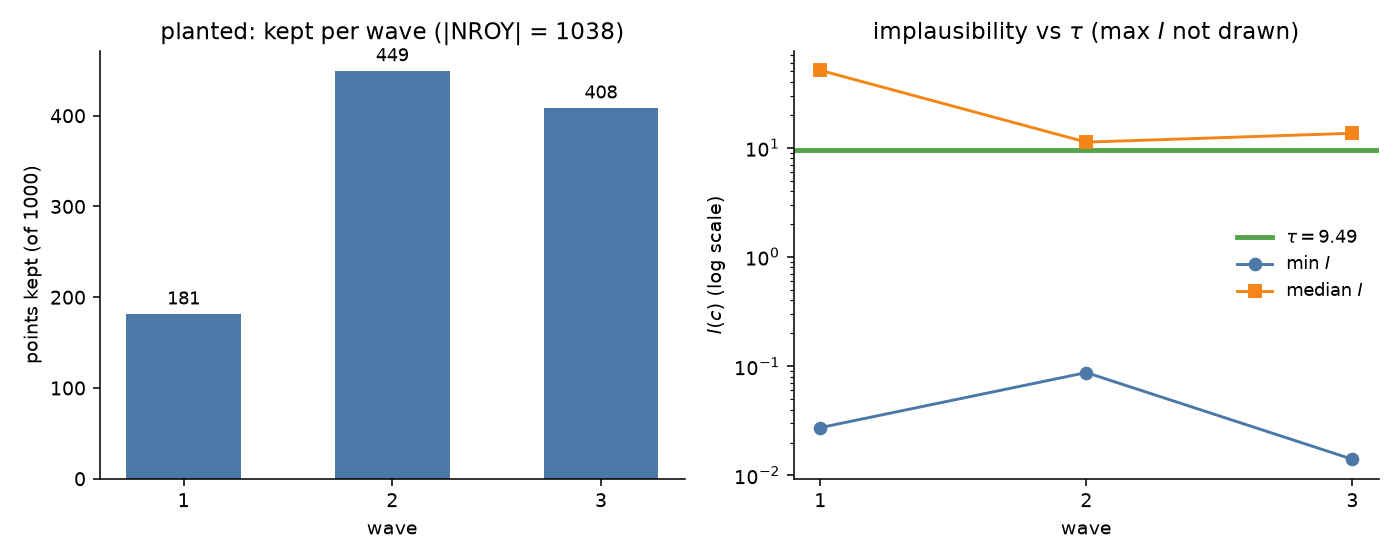
\includegraphics[width=\linewidth]{waves.png}
\captionof{figure}{Planted history matching. Left: points kept in each
wave. Right: min and median $I(c)$ against the threshold $\tau$ (log
scale). Later waves concentrate on the kept region. The threshold does
not move.}
\label{fig:waves}
\end{minipage}
\end{center}

\subsection{Which parameters the targets restrict}
\label{sec:spread}
For each parameter, the code divides the standard deviation over the
\ThetaSample{} sampled NROY points by the standard deviation of a
uniform draw over $C$ on that axis. A ratio near one means the moments
do not restrict that parameter. This readout was declared before the run
and is not a gate.
\begin{center}
\small
\begin{tabular}{@{}lccccc@{}}
\toprule
 & $\alpha$ & $\beta$ & $\gamma$ & $\kappa$ & $\sigma_\varepsilon$ \\
\midrule
spread ratio & \SpreadRatioAlpha & \SpreadRatioBeta & \SpreadRatioGamma & \SpreadRatioKappa & \SpreadRatioSigma \\
\bottomrule
\end{tabular}
\end{center}
Only $\alpha$ is pinned down. The ratios for $\beta$, $\gamma$ and
$\kappa$ are close to one, and $\sigma_\varepsilon$ is in between. The
peer weight $\gamma$ is the case the design most wanted to restrict
(through \texttt{sq\_peer\_corr}), and its ratio is \SpreadRatioGamma.
That is below one only in the third decimal, so in practice the
moments leave $\gamma$ open. The pre-registration expected a ratio
below one for $\gamma$ through the peer-correlation moment, and expected the pilot moment to restrict the trade-off between $\alpha$ and
$\kappa$ more than the earlier design did. This paper does not rerun the earlier design, so it cannot
check the second expectation against it. The sampled correlation between $\alpha$ and $\kappa$ is
\SpreadCorrAlphaKappa, and the one between $\alpha$ and $\gamma$ is
\SpreadCorrAlphaGamma. We report what the code found. The expectation on $\gamma$ was not met:
the ratio is below one only in the third decimal, and a spread ratio of
\SpreadRatioGamma{} is not a restriction.

\subsection{The image of \texorpdfstring{$\theta_2$}{theta2} is not a point}
At the planted point, $\theta_1(c^\star)=\ThetaOneStar$ and $\theta_2(c^\star)=\ThetaTwoStar$, and the premium is $\prem(c^\star)=\PremiumStar$. In this
model, seeding the highest-degree people barely beats seeding at random,
but that is a fact about this $c^\star$, not a theorem about targeting. The
spillover at $c^\star$ is $\dspill(c^\star)=\SpillStar$.

Over the \ThetaSample{} sampled NROY points, the headline image is $\Theta_{\hm}=[\ThetaHmLo,\,\ThetaHmHi]$,
and the image of the spillover is $\Theta_{\expset}=[\ThetaExpLo,\,\ThetaExpHi]$. The honest report for $\theta_2$ is the
range, not \ThetaTwoStar. The range is not a sampling distribution and
not a posterior.

\paragraph{Why the image is wide.}
The width of $\Theta_{\hm}$ is largely the assumption $\delta$. With
$\delta_1=\DeltaOne$ on a level moment, the rule lets each of the two levels
miss by about $\sqrt{\tau\delta_1^2}$, with $\tau=\Tau$. That allowance is
larger than $\theta_1(c^\star)=\ThetaOneStar$ itself, so the pilot level cannot
pin $\kappa$. The spread ratio for $\kappa$,
\SpreadRatioKappa, is what we would expect if the allowance covers the
effect of $\kappa$ on the pilot level, and Section~\ref{sec:menu} tests
that reading by shrinking $\delta_1$. The peer weight $\gamma$ is a
different case. Its ratio, \SpreadRatioGamma, is no restriction, and a
check at $c^\star$ found that the peer-correlation moment hardly moves across the
$\gamma$ range of the box. That check is not a committed result. The count of
moments is not the reason for the width.

Figure~\ref{fig:points} shows every sampled point. Each bar is a
pointwise Monte Carlo SE at a fixed $c$. For $\theta_2$ the bars are
smaller than the dots. For $\dspill$ they are visible.

\begin{center}
\begin{minipage}{\linewidth}
\centering
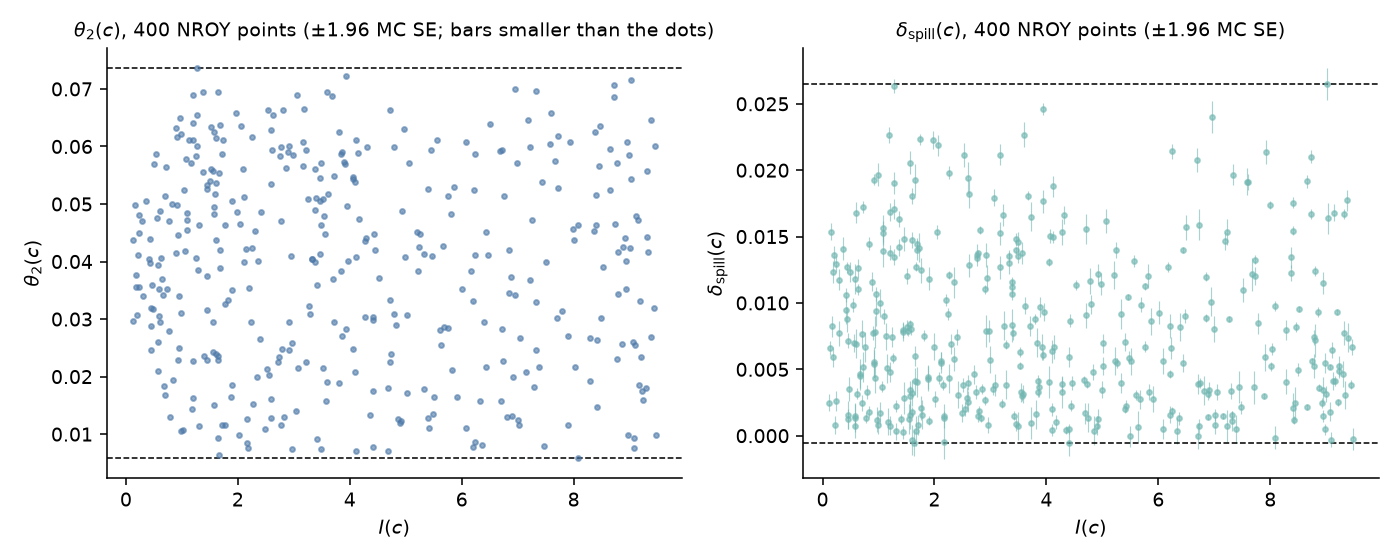
\includegraphics[width=\linewidth]{image_points.png}
\captionof{figure}{The \ThetaSample{} sampled NROY points against $I(c)$. Left:
$\theta_2(c)$. Right: $\dspill(c)$. Bars show $\pm1.96$ pointwise MC SE.
Dashed lines mark the image endpoints.}
\label{fig:points}
\end{minipage}
\end{center}

\paragraph{The endpoint recheck.}
The code evaluates again each point that sets an endpoint. It uses \RepsEstimand{}
fresh reps on separate streams. Table~\ref{tab:recheck} gives the
result.
\needspace{8\baselineskip}
\begin{center}
\small
\captionof{table}{Independent recheck of the endpoint candidates (SE is
the pointwise MC SE).}
\label{tab:recheck}
\begin{tabular}{@{}lccc@{}}
\toprule
endpoint & NROY index & pilot (SE) & fresh (SE) \\
\midrule
$\Theta_{\hm}$ lower & \RecheckHmLoIndex{} & $\RecheckHmLoPilot$ (\RecheckHmLoPilotSE) & $\RecheckHmLoFresh$ (\RecheckHmLoFreshSE) \\
$\Theta_{\hm}$ upper & \RecheckHmHiIndex{} & $\RecheckHmHiPilot$ (\RecheckHmHiPilotSE) & $\RecheckHmHiFresh$ (\RecheckHmHiFreshSE) \\
$\Theta_{\expset}$ lower & \RecheckExpLoIndex{} & $\RecheckExpLoPilot$ (\RecheckExpLoPilotSE) & $\RecheckExpLoFresh$ (\RecheckExpLoFreshSE) \\
$\Theta_{\expset}$ upper & \RecheckExpHiIndex{} & $\RecheckExpHiPilot$ (\RecheckExpHiPilotSE) & $\RecheckExpHiFresh$ (\RecheckExpHiFreshSE) \\
\bottomrule
\end{tabular}
\end{center}
Each bar in \texttt{image\_points.json} is a pointwise Monte Carlo SE
conditional on a fixed parameter point $c$. The displayed image
endpoints are extrema selected from \ThetaSample{} noisy estimates. So the SE
attached to the extremizing point is not an SE for the endpoint. It
does not include extremum-selection uncertainty. Fresh independent
re-evaluation of the pilot-selected extremizers removes reuse-of-noise
bias for those candidates. It is not simultaneous inference for the true
extrema, and it says nothing about extrema that the sample missed.

\subsection{The overlay: three points}
Figure~\ref{fig:overlay} puts each interval next to its own image at the
three diagnostic points. The rows are the min-I point, the median-I
point and $c^\star$, the village. The left column shows $\theta_2$ against $\Theta_{\hm}$ with the Foil~1 interval,
and the right column shows $\dspill$ against $\Theta_{\expset}$ with the Foil~2 interval. A
star marks the truth at that point, and a triangle marks the truth at
$c^\star$ (it is omitted in the $c^\star$ row, where it would sit under the star).

\begin{center}
\begin{minipage}{\linewidth}
\centering
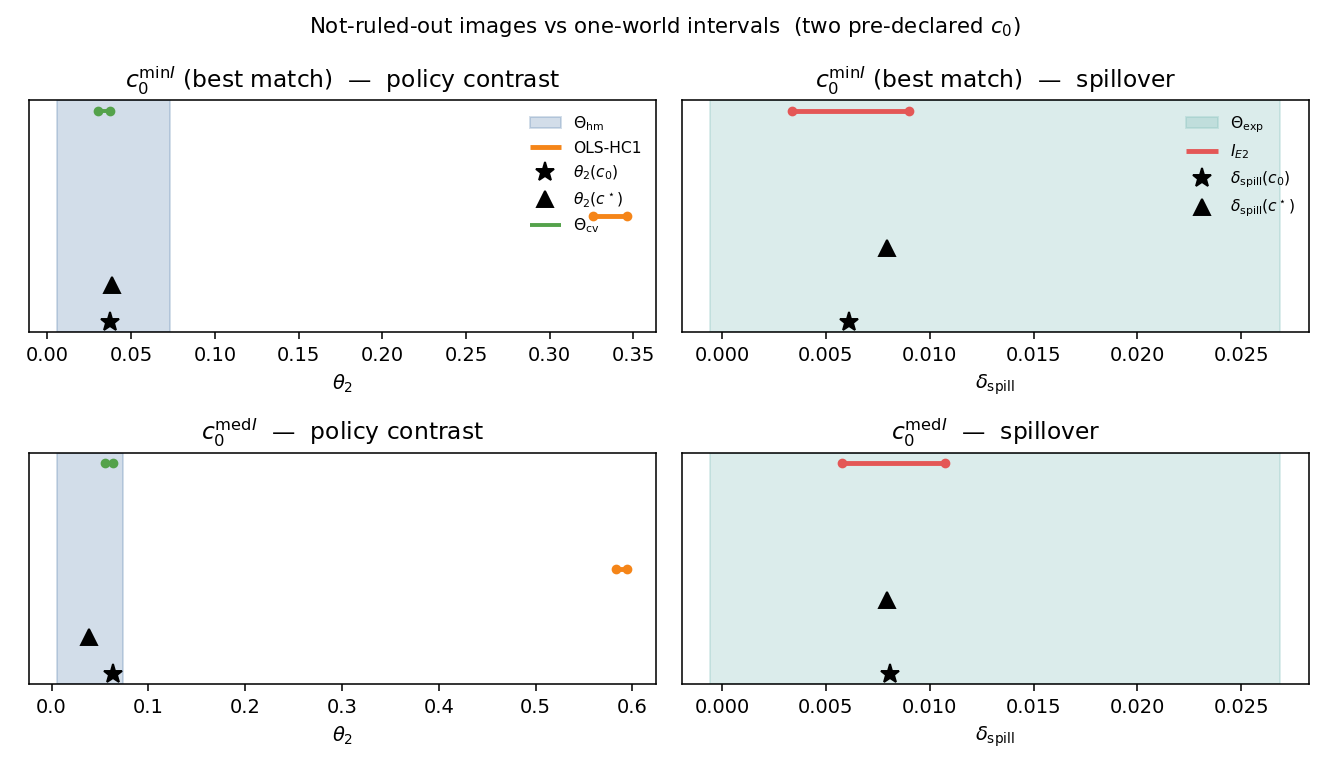
\includegraphics[width=\linewidth]{overlay.png}
\captionof{figure}{Images and one-world intervals at the three diagnostic
points. Left: $\theta_2$ against $\Theta_{\hm}$ with Foil~1. Right:
$\dspill$ against $\Theta_{\expset}$ with Foil~2. Each interval is
compared with its own image.}
\label{fig:overlay}
\end{minipage}
\end{center}

\needspace{22\baselineskip}
\begin{center}
\small
\setlength{\tabcolsep}{4pt}
\captionof{table}{The two foils at the three points. The first column
is the field experimenter, and the other two are the calibrator.}
\label{tab:foils}
\begin{tabular}{@{}lccc@{}}
\toprule
 & $c^\star$ (village) & min-I ($I=\MinI$) & median-I ($I=\MedI$) \\
\midrule
truth $\theta_2(c_0)$ & \ThetaTwoStar{} & \MinIThetaTwo{} & \MedIThetaTwo{} \\
Foil 1 interval $\Jone$ & $[\StarPtFoilOneLo,\,\StarPtFoilOneHi]$ & $[\MinIFoilOneLo,\,\MinIFoilOneHi]$ & $[\MedIFoilOneLo,\,\MedIFoilOneHi]$ \\
Foil 1 verdict & \StarPtFoilOneVerdict & \MinIFoilOneVerdict & \MedIFoilOneVerdict \\
contains truth at $c_0$ (a) & \StarPtFoilOneCoversTruth & \MinIFoilOneCoversTruth & \MedIFoilOneCoversTruth \\
contains truth at $c^\star$ (b) & \StarPtFoilOneCoversPlanted & \MinIFoilOneCoversPlanted & \MedIFoilOneCoversPlanted \\
\addlinespace
truth $\dspill(c_0)$ & \SpillStar{} & \MinISpill{} & \MedISpill{} \\
Foil 2 estimate (SE) & \StarPtFoilTwoEst{} (\StarPtFoilTwoSE) & \MinIFoilTwoEst{} (\MinIFoilTwoSE) & \MedIFoilTwoEst{} (\MedIFoilTwoSE) \\
Foil 2 interval $\Jtwo$ & $[\StarPtFoilTwoLo,\,\StarPtFoilTwoHi]$ & $[\MinIFoilTwoLo,\,\MinIFoilTwoHi]$ & $[\MedIFoilTwoLo,\,\MedIFoilTwoHi]$ \\
Foil 2 verdict (pilot image) & \StarPtFoilTwoVerdict & \MinIFoilTwoVerdict & \MedIFoilTwoVerdict \\
contains truth at $c_0$ (a) & \StarPtFoilTwoCoversTruth & \MinIFoilTwoCoversTruth & \MedIFoilTwoCoversTruth \\
contains truth at $c^\star$ (b) & \StarPtFoilTwoCoversPlanted & \MinIFoilTwoCoversPlanted & \MedIFoilTwoCoversPlanted \\
\bottomrule
\end{tabular}
\end{center}

\subsection{What the two analysts find}
\paragraph{The field experimenter, at $c^\star$.}
Her Foil~1 interval is $[\StarPtFoilOneLo,\,\StarPtFoilOneHi]$ and the truth is \ThetaTwoStar,
so the interval misses it, and the point estimate is \StarPtFoilOneBelowPct\% below the truth. Her interval
is also strictly inside $\Theta_{\hm}$. The failure
needs no calibration: it is layer~(a), and it comes from the
identification conditions of the estimator. Her Foil~2 interval
$[\StarPtFoilTwoLo,\,\StarPtFoilTwoHi]$ contains the spillover
\SpillStar. It starts below the lower end of $\Theta_{\expset}$, so
against the image it has no verdict.

\paragraph{The calibrator, at min-I and median-I.}
At both points the Foil~1 interval misses the truth at its own point
(layer~(a)) and the truth at the village (layer~(b)), and it sits strictly
inside the image. The Foil~2 interval contains the truth at its own
point and the truth at the village, and it also sits strictly inside the
image. At the median-I point the truth at the working point, $\theta_2=\MedIThetaTwo$,
differs from the truth at the village, $\theta_2(c^\star)=\ThetaTwoStar$, so
the assumption ``my world is the world'' is costly there. At the min-I point
the two are close ($\MinIThetaTwo$ and $\ThetaTwoStar$), but the median-I point
shows that membership in NROY does not guarantee it.

\paragraph{Containment and verdict are different tests.}
For Foil~2 they disagree. The interval contains the truth at every
point, and yet at both calibrated points it is F-OVERCONF. There is no
contradiction. An interval answers a question about one world, and the image
answers a question about all the worlds that the targets cannot rule out. A one-world
interval can be correct about its own world and narrower than the image at the same time. The
calibrator who reports that interval as her uncertainty about the village
would understate the uncertainty that the targets leave open. She happens to be right in this
realization, and the image is what tells her she might not have been.

\subsection{Foil 1: the SUTVA analyst}
Table~\ref{tab:foils} shows that the Foil 1 interval is narrow. At $c^\star$,
$\hat\beta=\StarPtBetaHat$ with interval $[\StarPtBetaLo,\,\StarPtBetaHi]$. At the
min-I point, $\hat\beta=\MinIBetaHat$ with interval $[\MinIBetaLo,\,\MinIBetaHi]$, and at the median-I point, $\hat\beta=\MedIBetaHat$ with
interval $[\MedIBetaLo,\,\MedIBetaHi]$. The scale factor is $k/N=\SeedShare$, and five statements stay with
every report of Foil~1.
\begin{enumerate}
  \item Foil 1 is not an identified estimator of the simulator's
        $\theta_2$ under the actual interference model. It is the
        whole-village policy estimate implied by a SUTVA analyst,
        $(k/N)\hat\beta$, with $k/N=\SeedShare$.
  \item That interpretation assumes consistency/SUTVA, conditional
        exchangeability and positivity given $X$, a correctly specified
        additive constant-effect outcome model, and a
        sampling/asymptotic basis for HC1. The deterministic top-degree
        assignment does not establish those assumptions.
  \item After scaling, the Foil 1 intervals are strictly inside
        $\Theta_{\hm}$ and exclude the truth at their own point at all three diagnostic points. So
        F-OVERCONF is an assumption-contingent
        interval-geometry finding. It is not a coverage claim for
        $\theta_2$ under interference.
  \item Across \RepsEstimand{} paired panels, about \UnseededShareMeanBetaPct\% of the gap between
        $\theta_2$ and $(k/N)$ times the \RepsEstimand-panel mean OLS
        coefficient is the policy effect on unseeded people. For the
        displayed replication-0 point estimate, the corresponding
        shares are about \StarPtUnseededShareDisplayedPct\% at $c^\star$, \MinIUnseededShareDisplayedPct\% at min-I and \MedIUnseededShareDisplayedPct\% at median-I.
  \item The rescaling was adopted after the frozen numbers were
        inspected. Its justification is the SUTVA aggregation identity.
        The post hoc design correction is disclosed.
\end{enumerate}

\paragraph{The gap decomposition.}
With paired streams, the policy effect splits exactly into a seeded
part and an unseeded part. Let $S$ be the seeded set, and let $y_2-y_0$
be the effect on a person in one rep. Then
\begin{equation}
  \theta_2
  = \underbrace{\tfrac{1}{N}\textstyle\sum_{i\in S}(y_2-y_0)}_{\text{the seeded part}}
  + \underbrace{\tfrac{1}{N}\textstyle\sum_{i\notin S}(y_2-y_0)}_{\text{the unseeded part}}.
\end{equation}
The unseeded part is zero under SUTVA. The seeded policy contrast is the
mean of $y_2-y_0$ over $S$, and under interference it is not a SUTVA effect of
own treatment. Table~\ref{tab:gap} gives the numbers. The gap for the
mean beta averages over \RepsEstimand{} panels, whereas the gap for the
displayed beta uses the one panel that Foil~1 sees. We keep the two
apart.
\needspace{20\baselineskip}
\begin{center}
\small
\setlength{\tabcolsep}{4pt}
\captionof{table}{Gap decomposition for Foil 1 (\RepsEstimand{} paired reps).}
\label{tab:gap}
\begin{tabular}{@{}lccc@{}}
\toprule
 & $c^\star$ & min-I point & median-I point \\
\midrule
$\theta_2$ & \ThetaTwoStar{} & \MinIThetaTwo{} & \MedIThetaTwo{} \\
seeded part & \StarPtSeededPart{} & \MinISeededPart{} & \MedISeededPart{} \\
unseeded part & \StarPtUnseededPart{} & \MinIUnseededPart{} & \MedIUnseededPart{} \\
seeded policy contrast & \StarPtSeededContrast{} & \MinISeededContrast{} & \MedISeededContrast{} \\
mean beta & \StarPtMeanBeta{} & \MinIMeanBeta{} & \MedIMeanBeta{} \\
gap for the mean beta & \StarPtGapMeanBeta{} & \MinIGapMeanBeta{} & \MedIGapMeanBeta{} \\
unseeded share of that gap & \StarPtUnseededShareMeanBeta{} & \MinIUnseededShareMeanBeta{} & \MedIUnseededShareMeanBeta{} \\
OLS-error part of that gap & \StarPtOlsErrorPart{} & \MinIOlsErrorPart{} & \MedIOlsErrorPart{} \\
gap for the displayed beta & \StarPtGapDisplayed{} & \MinIGapDisplayed{} & \MedIGapDisplayed{} \\
unseeded share of that gap & \StarPtUnseededShareDisplayed{} & \MinIUnseededShareDisplayed{} & \MedIUnseededShareDisplayed{} \\
baseline gap (seeded minus unseeded, $Y$ under control) & \StarPtBaselineGap{} & \MinIBaselineGap{} & \MedIBaselineGap{} \\
\bottomrule
\end{tabular}
\end{center}
Most of the gap is the effect on people who were not seeded, and a SUTVA
analyst has no term for it.

\paragraph{Why there is no forest foil.}
This was decision D3. In the degree arm, treatment is a deterministic function of degree and the index tie-break. Conditioning on degree leaves severe practical positivity failure: no treated people appear below degree \DegreeCut, no untreated people appear above degree \DegreeCut, and only one untreated person appears at degree \DegreeCut. Omitting degree leaves the assignment variable unadjusted. A forest can differ numerically from OLS, but it retains the same SUTVA blind spot and does not identify $\theta_2$ from this panel. A design-based third foil needs randomization across villages (Hudgens
and Halloran 2008, Baird et al.\ 2018).

\subsection{Foil 2: Hájek on the random arm}
\label{sec:foil2res}
At each diagnostic point, \texttt{covers\_truth} reports whether the displayed
interval contains the simulator truth at that point, and \texttt{covers\_planted\_truth} whether it contains the truth at $c^\star$.
Both are descriptive containment
indicators for that realized panel, not estimates of repeated-sampling
coverage and not validity gates. Foil 2 is checked separately by the
pre-declared repeated-assignment calibration in
\texttt{scripts/check\_foil2\_coverage.py}. All three Foil~2 intervals
contain both truths (Table~\ref{tab:foils}).

Against the saved \RepsEstimand-rep pilot image, $\Theta_{\expset}=[\ThetaExpLo,\,\ThetaExpHi]$,
the Foil 2 intervals at the min-I and median-I points,
$[\MinIFoilTwoLo,\,\MinIFoilTwoHi]$ and $[\MedIFoilTwoLo,\,\MedIFoilTwoHi]$, are strictly
interior and are classified F-OVERCONF. At $c^\star$ the interval reaches below the lower end of
$\Theta_{\expset}$, so there is no verdict.

Does the endpoint noise change these classifications? The independent
\RepsEstimand-rep recheck of the pilot-selected lower-end candidate
is \RecheckExpLoFresh{} (pointwise MC SE \RecheckExpLoFreshSE), against
\RecheckExpLoPilot{} in the pilot. The recheck of the upper-end candidate is
\RecheckExpHiFresh{} (SE \RecheckExpHiFreshSE), against \RecheckExpHiPilot. If we put the fresh values in
place of the pilot endpoints, the lower end of each calibrated interval is still above the lower
endpoint, the upper end is still below the upper endpoint, and the $c^\star$ interval
still starts below the lower endpoint. So none of the three classifications changes. This is a comparison of
printed numbers, not a field of the results. The recheck
evaluates selected candidates. It neither identifies nor bounds
the true extrema over all \ThetaSample{} sampled NROY points, and it does not
address an image that is too narrow.

An earlier version (commit \texttt{ebed7ce}) used a first-order variance that dropped
the covariance between the strata, and commit \texttt{36ed3e6} replaced it with the
Aronow--Samii variance.

\paragraph{The calibration check.}
The script \texttt{scripts/check\_foil2\_coverage.py} is a required check. Its gate uses outcomes that obey the
exposure map exactly, with a true spillover of \GateTruth, and it draws
\GateAssignments{} random-arm assignments. The gate rule was written
before the run: the gate fails if the ratio of the mean estimated
variance to the empirical variance, plus 1.645 bootstrap SE, is below 1.
The gate passes, with a mean estimate of \GateMeanEstimate{} and a ratio
of \GateRatio{} (bootstrap SE \GateRatioBootSE). The result:

\begin{quote}
In a fixed-world repeated-assignment check whose outcomes obey the
exposure map exactly, the nominal \ConfidencePct\% Foil 2 Wald interval covered
\GateCoveragePct\% of assignments (exact 95\% binomial interval \GateCoverageLoPct\%--\GateCoverageHiPct\%). The
average estimated variance was \GateRatio{} times the empirical design
variance, so the shortfall is not explained by average variance
underestimation. It reflects the finite-sample behavior of this
studentized normal interval, with the implemented Hájek linearization
and simulated joint exposure probabilities.
\end{quote}
The check is specific to this implementation. It is not a test of the
Aronow--Samii theorem. Their exact result is for Horvitz--Thompson
totals with exact joint probabilities. The code uses Hájek means, a
first-order linearization and one simulated table of joint
probabilities.

The script also reports the kernel, where the exposure map is not
exact because spillover also travels two steps. Over \CheckPanels{} kernel panels,
the coverage of the nominal \ConfidencePct\% interval is \KernelCovStar{} at $c^\star$, \KernelCovMinI{}
at the min-I point and \KernelCovMedI{} at the median-I point. If we redraw only
the assignment and hold the noise fixed, the coverage is \DesignCovStar, \DesignCovMinI{}
and \DesignCovMedI. The code reports these numbers but does not gate on them.
The gate result and these numbers are the only coverage numbers in the paper.

\subsection{A menu of assumptions (amendment A1)}
\label{sec:menu}
\emph{This subsection was decided after the v2 results were known.}
Amendment A1 of the pre-registration (\texttt{docs/preregistration-v2.md}) was
written once the main run had reported $\Theta_{\hm}$ and the spread ratios,
and once we had set the allowance $\sqrt{\tau\delta_1^2}$ beside
$\theta_1(c^\star)$. It does not test a hypothesis, and it is not a way to
choose $\delta$. The main design and every result above stay at
$\delta_1=\MenuDeltaMainLevel$. The menu shows how the image depends on the
assumption that appears to bind.

The menu sets the discrepancy of the two level moments to
\MenuDeltaMainLevel{} (Main), \MenuDeltaHalfLevel{} (Half) or
\MenuDeltaQuarterLevel{} (Quarter). The two correlation moments keep
$\delta=\DeltaTwo$. For each entry the code reruns the waves with the same
seed, NROY, the \ThetaSample-point image sample and the spread ratios. The
threshold $\tau$, the box $C$, the targets and every seed are unchanged.
The Main entry reproduces the main run exactly, and the script stops with an
error if it does not. The foils are not rerun at the calibrator's points,
because those points move with $\delta$. The field experimenter's intervals
at $c^\star$ do not depend on $\delta$, so we only classify them against each
entry's images.

\begin{center}
\small
\captionof{table}{The image under three level tolerances (amendment A1,
decided after the v2 results).}
\label{tab:menu}
\begin{tabular}{@{}lcccc@{}}
\toprule
entry & $\delta_1$ & $|\NROY|$ & $\Theta_{\hm}$ & $\Theta_{\expset}$ \\
\midrule
Main & \MenuDeltaMainLevel & \MenuDeltaMainNNroy & $[\MenuDeltaMainThetaHmLo,\,\MenuDeltaMainThetaHmHi]$ & $[\MenuDeltaMainThetaExpLo,\,\MenuDeltaMainThetaExpHi]$ \\
Half & \MenuDeltaHalfLevel & \MenuDeltaHalfNNroy & $[\MenuDeltaHalfThetaHmLo,\,\MenuDeltaHalfThetaHmHi]$ & $[\MenuDeltaHalfThetaExpLo,\,\MenuDeltaHalfThetaExpHi]$ \\
Quarter & \MenuDeltaQuarterLevel & \MenuDeltaQuarterNNroy & $[\MenuDeltaQuarterThetaHmLo,\,\MenuDeltaQuarterThetaHmHi]$ & $[\MenuDeltaQuarterThetaExpLo,\,\MenuDeltaQuarterThetaExpHi]$ \\
\bottomrule
\end{tabular}

\vspace{0.8em}
\captionof{table}{Spread ratios and the field experimenter's verdicts at
$c^\star$ under the same entries. Finding is the history-matching finding
(\texttt{finding\_hm}).}
\label{tab:menu2}
\begin{tabular}{@{}lcccccc@{}}
\toprule
entry & $\alpha$ & $\kappa$ & $\gamma$ & finding & Foil 1 at $c^\star$ & Foil 2 at $c^\star$ \\
\midrule
Main & \MenuDeltaMainSpreadRatioAlpha & \MenuDeltaMainSpreadRatioKappa & \MenuDeltaMainSpreadRatioGamma & \MenuDeltaMainFinding & \MenuDeltaMainFoilOneVerdict & \MenuDeltaMainFoilTwoVerdict \\
Half & \MenuDeltaHalfSpreadRatioAlpha & \MenuDeltaHalfSpreadRatioKappa & \MenuDeltaHalfSpreadRatioGamma & \MenuDeltaHalfFinding & \MenuDeltaHalfFoilOneVerdict & \MenuDeltaHalfFoilTwoVerdict \\
Quarter & \MenuDeltaQuarterSpreadRatioAlpha & \MenuDeltaQuarterSpreadRatioKappa & \MenuDeltaQuarterSpreadRatioGamma & \MenuDeltaQuarterFinding & \MenuDeltaQuarterFoilOneVerdict & \MenuDeltaQuarterFoilTwoVerdict \\
\bottomrule
\end{tabular}
\end{center}

The tolerance matters most for $\kappa$ and $\alpha$. The sampled NROY set
shrinks as $\delta_1$ falls, and at Quarter both images are narrower than at
Main. The spread ratio for $\kappa$ falls to
\MenuDeltaQuarterSpreadRatioKappa{} and the one for $\alpha$ to
\MenuDeltaQuarterSpreadRatioAlpha, which fits the reading that the level
allowance is what leaves $\kappa$ open. The ratio for $\gamma$ stays near one
(\MenuDeltaQuarterSpreadRatioGamma{} at Quarter), but the menu leaves the
correlation tolerance alone, so it says nothing new about the $\gamma$
expectation. The entries are not nested: the upper end of both images at
Half sits above the one at Main, because each image is the range over a
\ThetaSample-point sample from a different finite NROY set, with the waves
redrawn on it. We do not read small moves of an endpoint as a trend. The
clear change is at Quarter. There the lower end of $\Theta_{\expset}$ is
above zero (\MenuDeltaQuarterThetaExpLo), whereas under Main and Half the
sign of the spillover is open.

The verdicts do not move. At $c^\star$, Foil~1 is
\MenuDeltaMainFoilOneVerdict{} at every entry, and Foil~2 has
\MenuDeltaMainFoilTwoVerdict{} at every entry, as in the main run. No entry
returns F-EMPTY or F-SINGLETON; the finding is \MenuDeltaMainFinding{} at each.
A smaller $\delta_1$ does not hand Foil~2 a verdict at $c^\star$, even
at Quarter, where the lower end of $\Theta_{\expset}$ has left zero.

The menu is the reporting rule of Tamer (2010) applied to $\delta$: a set
under each of several assumptions, instead of one answer. The trade is the
one of Section~\ref{sec:pi}. A smaller $\delta_1$ is a stronger assumption,
namely that the kernel matches the targets more closely. It gives a smaller
set, and it asks the reader to believe more. In this planted exercise the
targets are the simulator's own output, so the smaller tolerances are not an
unfounded claim here. With external targets, $\delta$ is the allowance for a
model that is not the world, and the claim would have to be defended. The
set is still not Tamer's identified set (Section~\ref{sec:not}); the idea
borrowed is the reporting rule. We adopt none of the entries, and the
results of this paper stay at Main.

%----------------------------------------------------------------
\section{Relation to partial identification}
\label{sec:pi}

This section is about the reporting logic only. Section~\ref{sec:not}
lists what the procedure is not.

\paragraph{Where the set comes from.}
In much of the partial-identification literature the set comes from an
incomplete model. A game with multiple equilibria does not say which
outcome occurs, so the model allows a set of outcomes, and the data
bound the parameters without pinning them down (Tamer 2003, 2010). The
set in this paper does not come from there. The kernel is complete:
for each $c$ and each draw of the noise it returns one panel, and
Section~\ref{sec:props} shows that the model has a unique stationary
regime. The set does not come from an incomplete kernel. It comes from targets
that do not restrict the parameters. Section~\ref{sec:spread} shows that
only $\alpha$ is pinned, and that $\sigma_\varepsilon$
(\SpreadRatioSigma) is only partly restricted. The count of moments,
\NMoments{} against five free parameters, is not the binding reason. The
level tolerance exceeds $\theta_1(c^\star)$, so the pilot cannot pin
$\kappa$, and the peer-correlation moment does not restrict $\gamma$.
Many complete worlds fit the same targets.

\paragraph{The image is a set under assumptions.}
The image is the set of effects under the maintained assumptions:
the kernel, the box $C$, $\delta$, the targets and $\tau$. Adding one
more assumption, $c=c_0$, collapses it to the single value
$\theta_2(c_0)$. That is what the calibrator does when she works at one
point. The trade is the one Manski (2003) calls the law of decreasing
credibility: a stronger assumption gives a sharper answer and a less
credible one. In Table~\ref{tab:foils} the sharper answer is the narrow
interval at one point, and the credibility cost is the gap between
$\theta_2(c_0)$ and $\theta_2(c^\star)$ at the median-I point.
Section~\ref{sec:menu} gives the same trade for $\delta$.

\paragraph{What the targets restrict.}
How much of the set the targets remove is measured, not assumed. The
spread ratios in Section~\ref{sec:spread} say which parameters the
moments restrict.

%----------------------------------------------------------------
\section{Who will care, and who will not}

Novelty at the level of slogans is weak. History matching already rules out
regions of input space and keeps the rest, the NROY set (Craig et al.\ 1997;
Vernon, Goldstein and Bower 2010). Equifinality, where different parameter
sets fit the data equally well, is not new in simulation modelling
(Beven 2006). Partial identification already
says: report the set. Interference already has overall and direct
effects (Halloran and Struchiner 1995; Hudgens and Halloran 2008). A regression with robust
standard errors already gives an interval for a given panel. None of
these pieces is new, so the remaining wedge is the composition: a named
policy contrast under interference is reported as the image of a
history-matched set, and two analysts are graded against it. The
simulator is planted, so the truth is known. That is enough for an
applied project, but it is not a methods paper.

\paragraph{Anyone who calibrates a simulator for policy.}
This matters if you publish a policy number from an agent-based model, a
structural model or a microsimulation. Today you probably report the
Monte Carlo error at one best parameter point. The overlay shows a split.
Sampling error at one point is not uncertainty about which points the
targets still allow. An empty sampled NROY is a usable negative result for the declared
design: the run found no sampled point that passed the threshold for
those targets. It does not establish infeasibility over all of $C$. You
must not loosen the threshold. The width of the image is measured, not assumed. Here
$\Theta_{\hm}=[\ThetaHmLo,\,\ThetaHmHi]$.

\paragraph{Empirical causal inference.}
This is not a new identification strategy: it does not replace
unconfoundedness, an instrument, difference-in-differences or a
regression discontinuity, and it does not estimate effects that vary by
covariate on a network. It does, however, matter in two narrow cases.

(1)~You use a model as the identification vehicle, and you quote one $\hat\theta$. The model can be structural, an epidemic simulator or an agent-based model of a campaign. The object to report is then the declared empirical image of
$\theta$ over the sampled NROY points. A one-world interval quantifies
within-point uncertainty under the analyst's stated assumptions. It is
not the image.

(2)~Interference is in the model, and the individual effect is not
defined. The well-posed object is a contrast of assignment rules. A
SUTVA analyst on a targeting arm, where $D$ is a function of the graph,
measures something near ``being a top-degree person.'' That is an
identification remark, not an estimator contest.

\paragraph{This project, specifically.}
The overlay is checkable because the targets were planted. The moments
are the kind a researcher could observe, a status quo and one pilot, but
the numbers are the simulator's own, so this is not an empirical
estimate of any real campaign, and we do not present it
as one. It shows that the composition can be run, with declared
verdicts, including F-EMPTY and no verdict. As a contribution to
empirical causal inference on real networks, it is a toy with a clean
dictionary of objects. It becomes more only if someone supplies targets
that this kernel can match, and those targets need a stated target
population and a transport model. The threshold $\tau$ must not move.

%----------------------------------------------------------------
\section{What the procedure is not}
\label{sec:not}

\begin{itemize}
  \item Not a posterior over $c$, and not a distribution of treatment
        effects. $\Theta_{\hm}$ comes from a thresholded discrepancy, in which
        sampling noise is folded into $V$ and the kernel is taken as
        true.
  \item Not a Manski or Tamer identified set. This is a finite
        empirical image produced by thresholding simulated moment
        discrepancies for a fully specified kernel. The analogy is only
        the reporting rule: do not collapse a set-valued result to one
        convenient point.
  \item Not a confidence set. A thresholded criterion function looks like
        the level sets of Chernozhukov, Hong and Tamer (2007), and the
        image of $\theta_2$ over such a set is a projection, the object of
        Imbens and Manski (2004) and Kaido, Molinari and Stoye (2019).
        Those papers give coverage guarantees under their
        assumptions. Nothing here claims one, and $V$ contains the
        discrepancy $\delta$, which is a tolerance and not a sampling variance.
  \item Not a calibrated test. The threshold $\tau$ is the
        \Confidence{} quantile of $\chi^2_{\NMoments}$, but $V$ is diagonal while
        the four moments are not independent: the control and random levels
        share a state stream. And $\delta^2$, not the sampling variance, fills
        $V$. So $\tau$ is a heuristic tolerance. It is not a test level, and
        $I(c^\star)$ sits far below it.
  \item Not independent of the targets. The foils' panel is rep~0, and rep~0
        is also one of the \RepsZ{} reps whose mean defines $z$. The foils
        therefore see data that helped set the targets. Rep~0 carries a
        weight of $1/\RepsZ$ in $z$, and we did not rerun the pipeline
        without it. We have not enumerated the rejected wave points that sit
        just above $\tau$, which would be the ones a small shift in $z$ could
        move into NROY.
  \item Not the same estimand for Foil~2 and its truth. The Hájek estimator
        targets the inverse-probability exposure contrast, and the truth is
        the mean of the unweighted realized stratum contrasts
        (Section~\ref{sec:design}). On this run they are close, and no
        containment flag depends on the difference. That is a fact about this
        kernel, not an identity, and it was not tested on another kernel.
  \item Not a guarantee that the image is wide: its width is measured,
        not assumed. The width is largely the assumption $\delta$
        (Section~\ref{sec:menu}).
  \item Not a claim that the closest NROY point recovers $c^\star$, which it
        does not: fit does not pick the truth.
  \item Not a coverage claim for either foil: F-OVERCONF is about interval
        geometry under the analyst's assumptions, and the containment flags
        describe one realized panel.
  \item Not a finding that analysts are bad at networks. Each
        quantifies within-point uncertainty under its own stated
        assumptions. The overlay asks whether
        one parameter point is enough.
  \item Not a claim about the real world: the project has one planted
        point, one graph and one set of targets, and it claims no
        external validity.
\end{itemize}

%----------------------------------------------------------------
\section*{References}
{\small\raggedright
\setlength{\parskip}{0.3em}
\noindent Aronow, P.~M. and C.~Samii (2017). Estimating average causal effects under general interference, with application to a social network experiment. \textit{Annals of Applied Statistics} 11(4), 1912--1947. \href{https://doi.org/10.1214/16-AOAS1005}{doi:10.1214/16-AOAS1005}

\noindent Baird, S., J.~A. Bohren, C.~McIntosh and B.~\"Ozler (2018). Optimal design of experiments in the presence of interference. \textit{Review of Economics and Statistics} 100(5), 844--860. \href{https://doi.org/10.1162/rest_a_00716}{doi:10.1162/rest\_a\_00716}

\noindent Beven, K. (2006). A manifesto for the equifinality thesis. \textit{Journal of Hydrology} 320(1--2), 18--36. \href{https://doi.org/10.1016/j.jhydrol.2005.07.007}{doi:10.1016/j.jhydrol.2005.07.007}

\noindent Bramoull\'e, Y., H.~Djebbari and B.~Fortin (2009). Identification of peer effects through social networks. \textit{Journal of Econometrics} 150(1), 41--55. \href{https://doi.org/10.1016/j.jeconom.2008.12.021}{doi:10.1016/j.jeconom.2008.12.021}

\noindent Brock, W.~A. and S.~N. Durlauf (2001). Discrete choice with social interactions. \textit{Review of Economic Studies} 68(2), 235--260. \href{https://doi.org/10.1111/1467-937X.00168}{doi:10.1111/1467-937X.00168}

\noindent Chernozhukov, V., H.~Hong and E.~Tamer (2007). Estimation and confidence regions for parameter sets in econometric models. \textit{Econometrica} 75(5), 1243--1284. \href{https://doi.org/10.1111/j.1468-0262.2007.00794.x}{doi:10.1111/j.1468-0262.2007.00794.x}

\noindent Craig, P.~S., M.~Goldstein, A.~H. Seheult and J.~A. Smith (1997). Pressure matching for hydrocarbon reservoirs: a case study in the use of Bayes linear strategies for large computer experiments. In \textit{Case Studies in Bayesian Statistics III}, Lecture Notes in Statistics 121, 37--93. Springer. \href{https://doi.org/10.1007/978-1-4612-2290-3_2}{doi:10.1007/978-1-4612-2290-3\_2}

\noindent Halloran, M.~E. and C.~J. Struchiner (1995). Causal inference in infectious diseases. \textit{Epidemiology} 6(2), 142--151. \href{https://doi.org/10.1097/00001648-199503000-00010}{doi:10.1097/00001648-199503000-00010}

\noindent Hudgens, M.~G. and M.~E. Halloran (2008). Toward causal inference with interference. \textit{Journal of the American Statistical Association} 103(482), 832--842. \href{https://doi.org/10.1198/016214508000000292}{doi:10.1198/016214508000000292}

\noindent Imbens, G.~W. and C.~F. Manski (2004). Confidence intervals for partially identified parameters. \textit{Econometrica} 72(6), 1845--1857. \href{https://doi.org/10.1111/j.1468-0262.2004.00555.x}{doi:10.1111/j.1468-0262.2004.00555.x}

\noindent Kaido, H., F.~Molinari and J.~Stoye (2019). Confidence intervals for projections of partially identified parameters. \textit{Econometrica} 87(4), 1397--1432. \href{https://doi.org/10.3982/ECTA14075}{doi:10.3982/ECTA14075}

\noindent Manski, C.~F. (1993). Identification of endogenous social effects: the reflection problem. \textit{Review of Economic Studies} 60(3), 531--542. \href{https://doi.org/10.2307/2298123}{doi:10.2307/2298123}

\noindent Manski, C.~F. (2003). \textit{Partial Identification of Probability Distributions.} Springer. \href{https://doi.org/10.1007/b97478}{doi:10.1007/b97478}

\noindent Tamer, E. (2003). Incomplete simultaneous discrete response model with multiple equilibria. \textit{Review of Economic Studies} 70(1), 147--165. \href{https://doi.org/10.1111/1467-937X.00240}{doi:10.1111/1467-937X.00240}

\noindent Tamer, E. (2010). Partial identification in econometrics. \textit{Annual Review of Economics} 2, 167--195. \href{https://doi.org/10.1146/annurev.economics.050708.143401}{doi:10.1146/annurev.economics.050708.143401}

\noindent Vernon, I., M.~Goldstein and R.~G. Bower (2010). Galaxy formation: a Bayesian uncertainty analysis. \textit{Bayesian Analysis} 5(4), 619--669. \href{https://doi.org/10.1214/10-BA524}{doi:10.1214/10-BA524}
}

\vspace{1.2em}
{\small
\noindent\textit{Implementation.}
Repo \texttt{ecn593-applied-project}, branch \texttt{main}.
\texttt{scripts/replicate.py} reruns everything. Each result file records
the commit that produced it (\texttt{git\_commit}).
$|\NROY|=\NNroy$,
$\Theta_{\hm}=[\ThetaHmLo,\,\ThetaHmHi]$,
$\theta_2(c^\star)=\ThetaTwoStar$.
Foil~1 is OLS-HC1 scaled by $k/N$.
Figures are redrawn from the saved results.
\texttt{README.md} lists the commands to replicate every number. The design is
frozen in \texttt{docs/preregistration-v2.md}.
}

\end{document}
